%        File: technology.tex
%     Created: Sun Mar 31 03:00 PM 2013 C
% Last Change: Sun Mar 31 03:00 PM 2013 C
%


%\documentclass[11pt,handout]{beamer}
\documentclass[9pt]{beamer}
\usetheme[white]{Wisconsin}
%\title[short title]{long title}
\title[Geologic Repositories and the Fuel Cycle]{Geologic Repositories and the Fuel Cycle}
%\subtitle[short subtitle]{long subtitle}
\subtitle[NPRE412]{NPRE412}
%\author[short name]{long name}
\author[Kathryn D. Huff]{Kathryn D. Huff}
%\date[short date]{long date}
\date[10.31.2016]{October 31, 2016}
%\institution[short name]{long name}
\institute[UIUC]{University of Illinois at Urbana-Champaign}

%\usepackage{bbding}
\usepackage{amsfonts}
\usepackage{amsmath}
\usepackage{graphicx}
\usepackage{subfigure}
\usepackage{booktabs} % nice rules for tables
\usepackage{microtype} % if using PDF
\usepackage{bigints}
\newcommand{\units}[1] {\:\text{#1}}%
\newcommand{\SN}{S$_N$}%{S$_\text{N}$}%{$S_N$}%
\DeclareMathOperator{\erf}{erf}

%page numbers
\setbeamertemplate{footline}[page number]
%Those icons in the references are terrible looking
\setbeamertemplate{bibliography item}[text]
\begin{document}
%%%%%%%%%%%%%%%%%%%%%%%%%%%%%%%%%%%%%%%%%%%%%%%%%%%%%%%%%%%%%
%% From uw-beamer Here's a handy bit of code to place at 
%% the beginning of your presentation (after \begin{document}):
\newcommand*{\alphabet}{ABCDEFGHIJKLMNOPQRSTUVWXYZabcdefghijklmnopqrstuvwxyz}
\newlength{\highlightheight}
\newlength{\highlightdepth}
\newlength{\highlightmargin}
\setlength{\highlightmargin}{2pt}
\settoheight{\highlightheight}{\alphabet}
\settodepth{\highlightdepth}{\alphabet}
\addtolength{\highlightheight}{\highlightmargin}
\addtolength{\highlightdepth}{\highlightmargin}
\addtolength{\highlightheight}{\highlightdepth}
\newcommand*{\Highlight}{\rlap{\textcolor{HighlightBackground}{\rule[-\highlightdepth]{\linewidth}{\highlightheight}}}}
%%%%%%%%%%%%%%%%%%%%%%%%%%%%%%%%%%%%%%%%%%%%%%%%%%%%%%%%%%%%%
%%--------------------------------%%
\frame{
  \titlepage
}

\section{Geologic Repository Concepts}
%%--------------------------------%%
\begin{frame}
  \frametitle{Outline}
  \tableofcontents[currentsection]
\end{frame}

\subsection{Components}


%%----------------------------------------%%
\begin{frame}[ctb!]
  \frametitle{Repository Components}
\footnotesize{
  \begin{figure}[htbp!]
  \begin{center}
    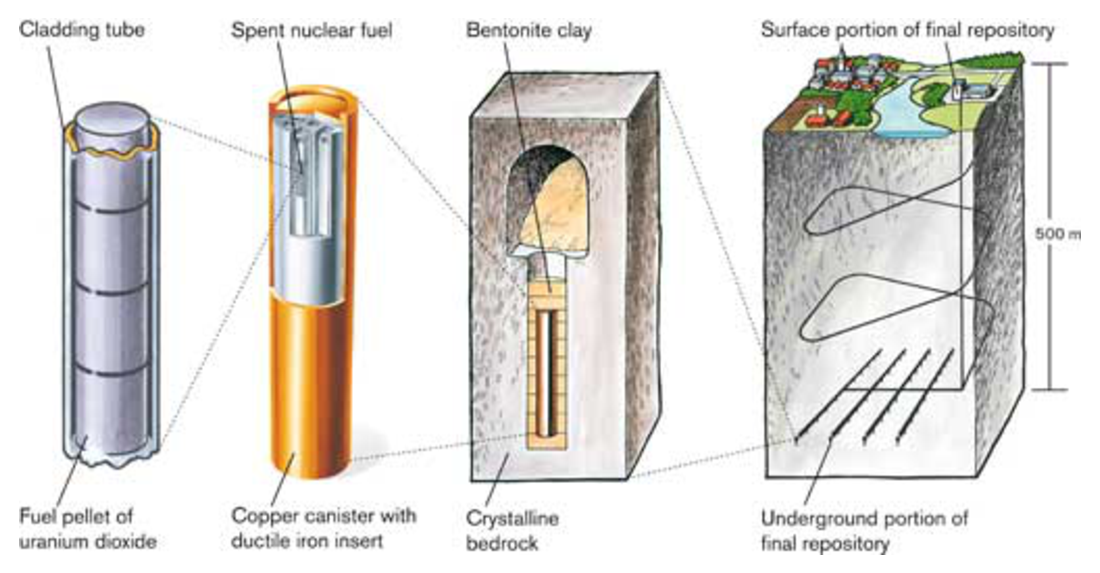
\includegraphics[width=0.7\textwidth]{skb_components.eps}
  \end{center}
  \caption{Geologic disposal systems typically employ engineered barrier 
    systems as well as natural barrier systems. This is a Swedish concept in 
    granite \cite{ab_long-term_2006}.}
  \label{fig:skb_components}
\end{figure}

}
\end{frame}

%%----------------------------------------%%
\begin{frame}[ctb!]
  \frametitle{Engineered Barriers : Waste Forms}
\footnotesize{
  The first line of defense is the waste form.
  \begin{figure}[htbp!]
  \begin{center}
    \includegraphics[width=0.7\textheight]{<++>.eps}
  \end{center}
  \caption{<++>\cite{<++>}.}
  \label{fig:<++>}
\end{figure}

}
\end{frame}

%%----------------------------------------%%
\begin{frame}[ctb!]
  \frametitle{Engineered Barriers : Waste Packages}
\footnotesize{
  \begin{figure}[htbp!]
  \begin{center}
    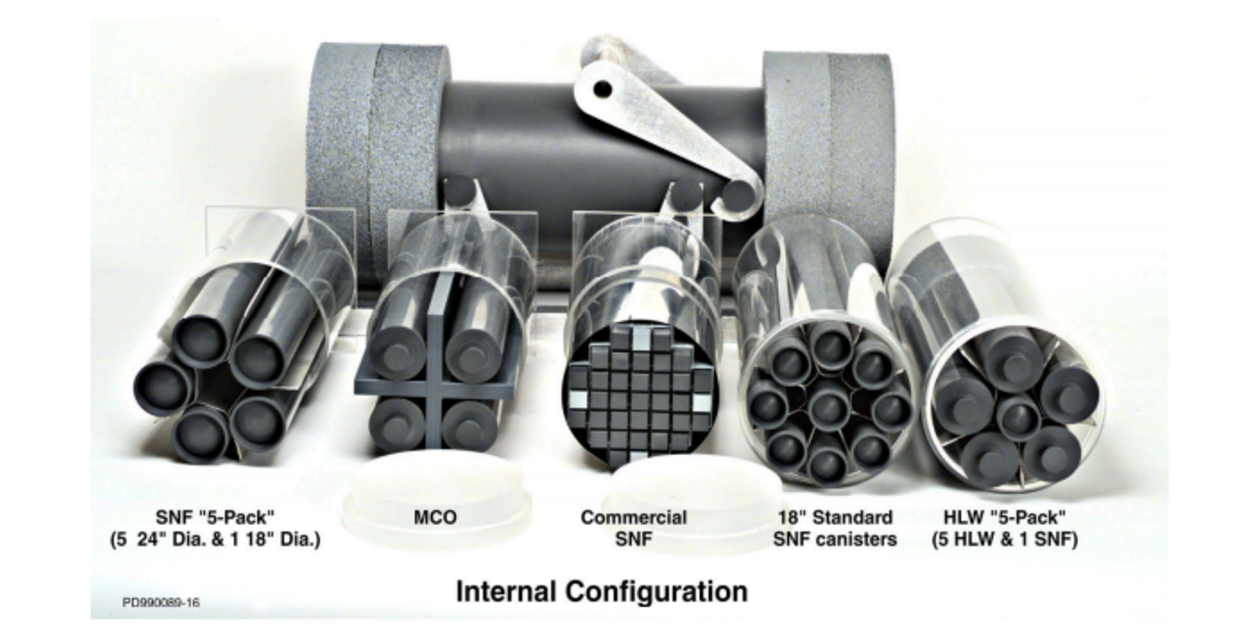
\includegraphics[width=0.7\textwidth]{packages_ineel.eps}
  \end{center}
  \caption{Conceptual mockup of waste packages around waste forms 
    \cite{bridges_standardized_2001}.}
  \label{fig:packages}
\end{figure}

}
\end{frame}

%%----------------------------------------%%
\begin{frame}[ctb!]
  \frametitle{Engineered Barriers : Disposal Cask}
\footnotesize{
  \begin{figure}[htbp!]
  \begin{center}
    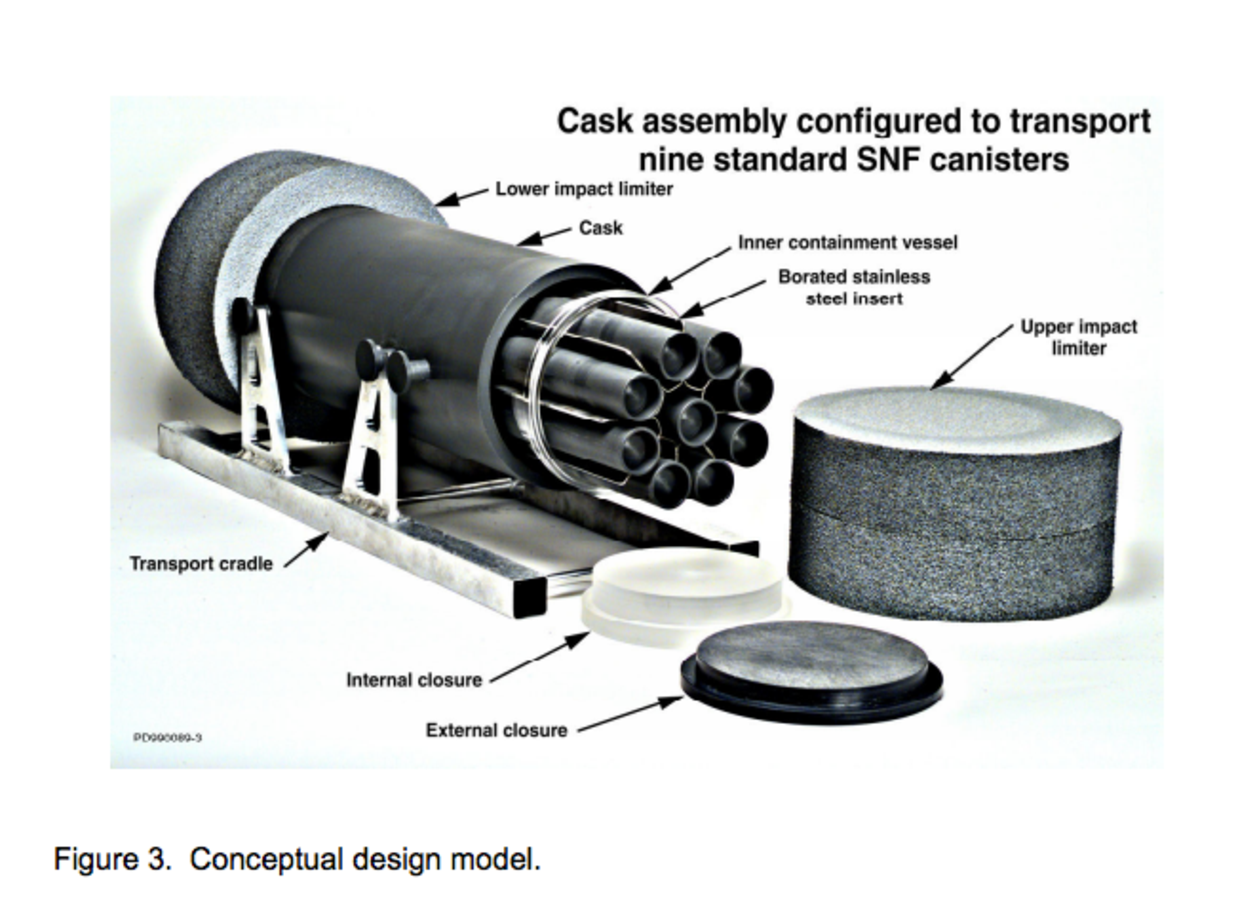
\includegraphics[width=0.7\textwidth]{cask_ineel.eps}
  \end{center}
  \caption{Conceptual mockup of a transport and disposal cask 
    \cite{bridges_standardized_2001}.}
  \label{fig:packages}
\end{figure}

}
\end{frame}

%%----------------------------------------%%
\begin{frame}[ctb!]
  \frametitle{Engineered Barriers : Tunnel}
\footnotesize{
  \begin{figure}[htbp!]
  \begin{center}
    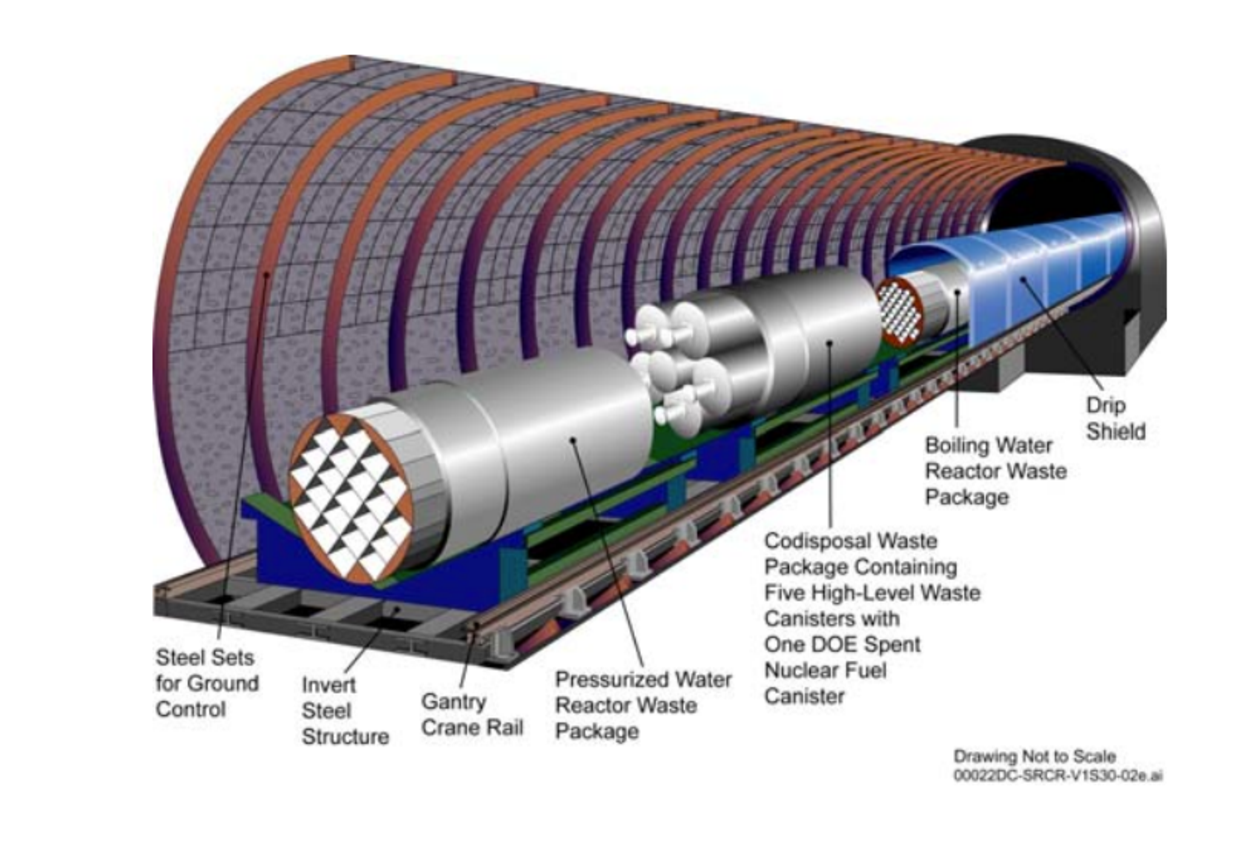
\includegraphics[height=0.7\textwidth]{yucca_tunnel.eps}
  \end{center}
  \caption{The current U.S. geologic disposal concept \cite{peters_whats_2013}.}
  \label{fig:yucca_tunnel}
\end{figure}

}
\end{frame}

%%----------------------------------------%%
\begin{frame}[ctb!]
  \frametitle{Natural Barrier : Geology}
\footnotesize{
  \begin{figure}[htbp!]
  \begin{center}
    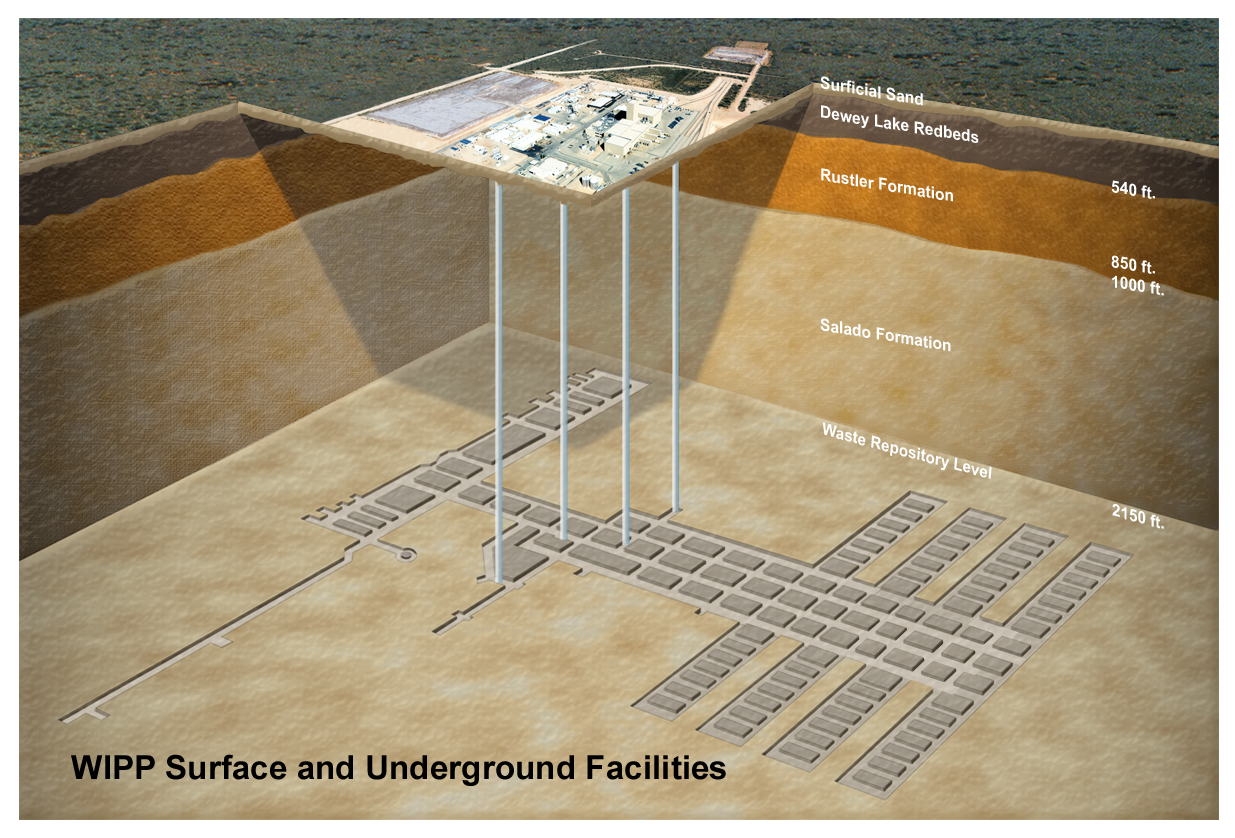
\includegraphics[width=0.7\textheight]{wipp_stratigraph.eps}
  \end{center}
  \caption{The Waste Isolation Pilot Plant has many geologic layers above the 
    salt bed \cite{doe_wipp_2013}.}
  \label{fig:wipp}
\end{figure}

}
\end{frame}

\subsection{Layouts}
\begin{frame}
  \frametitle{Repository Layouts}

  \begin{minipage}{0.49\textwidth}
    \begin{figure}[h!]
      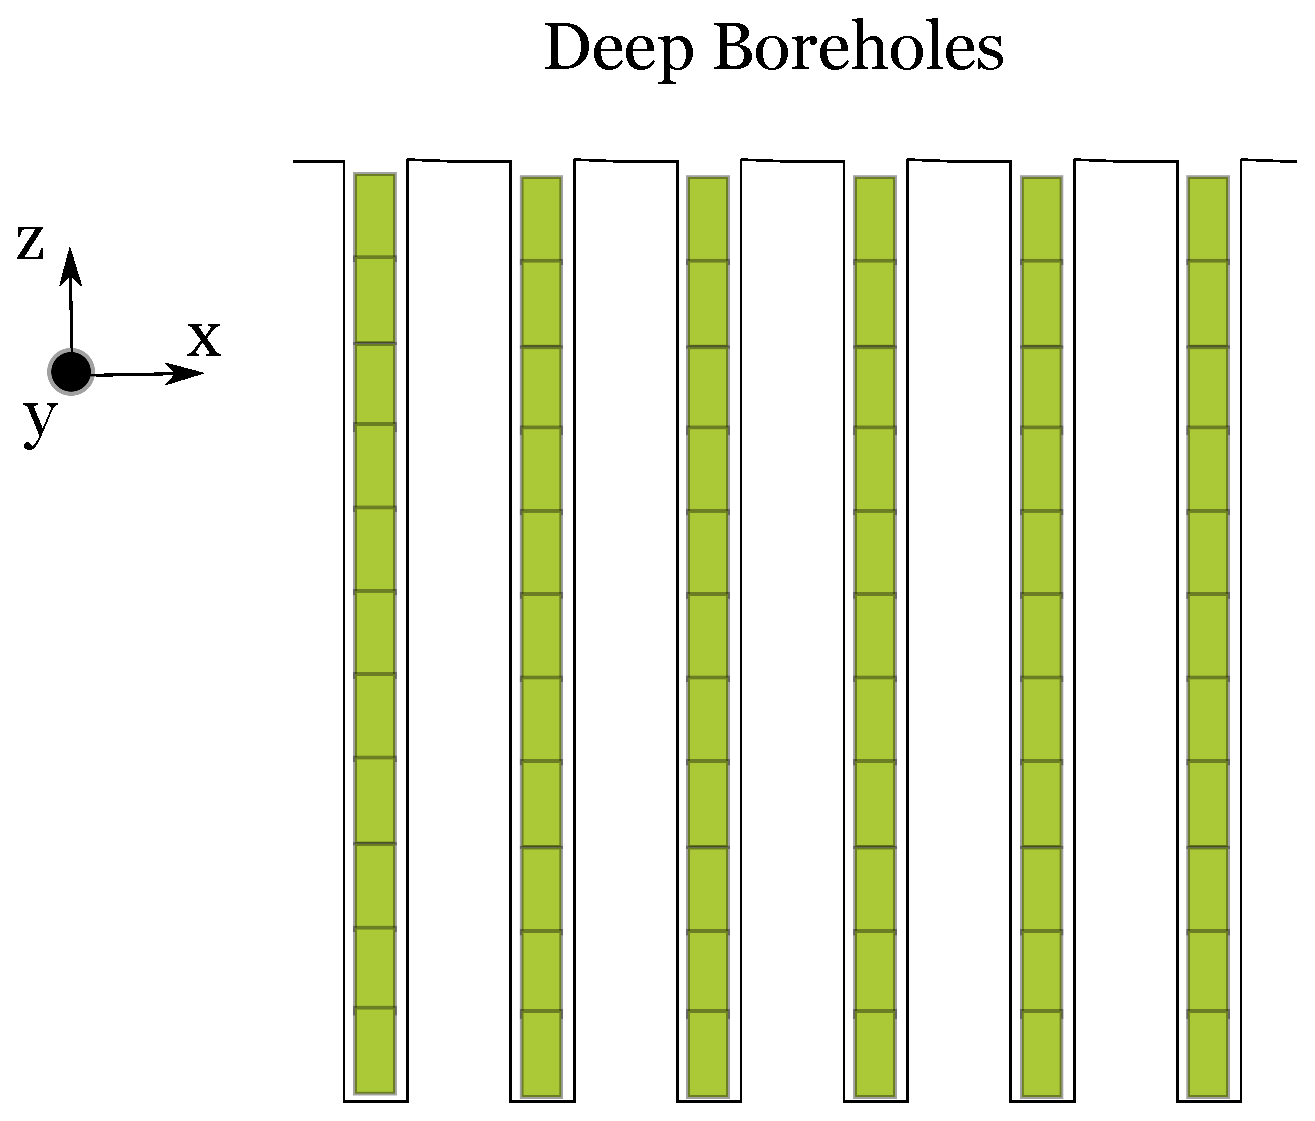
\includegraphics[width=0.75\textwidth]{boreholes.eps}
    \end{figure}
    \begin{figure}[h!]
      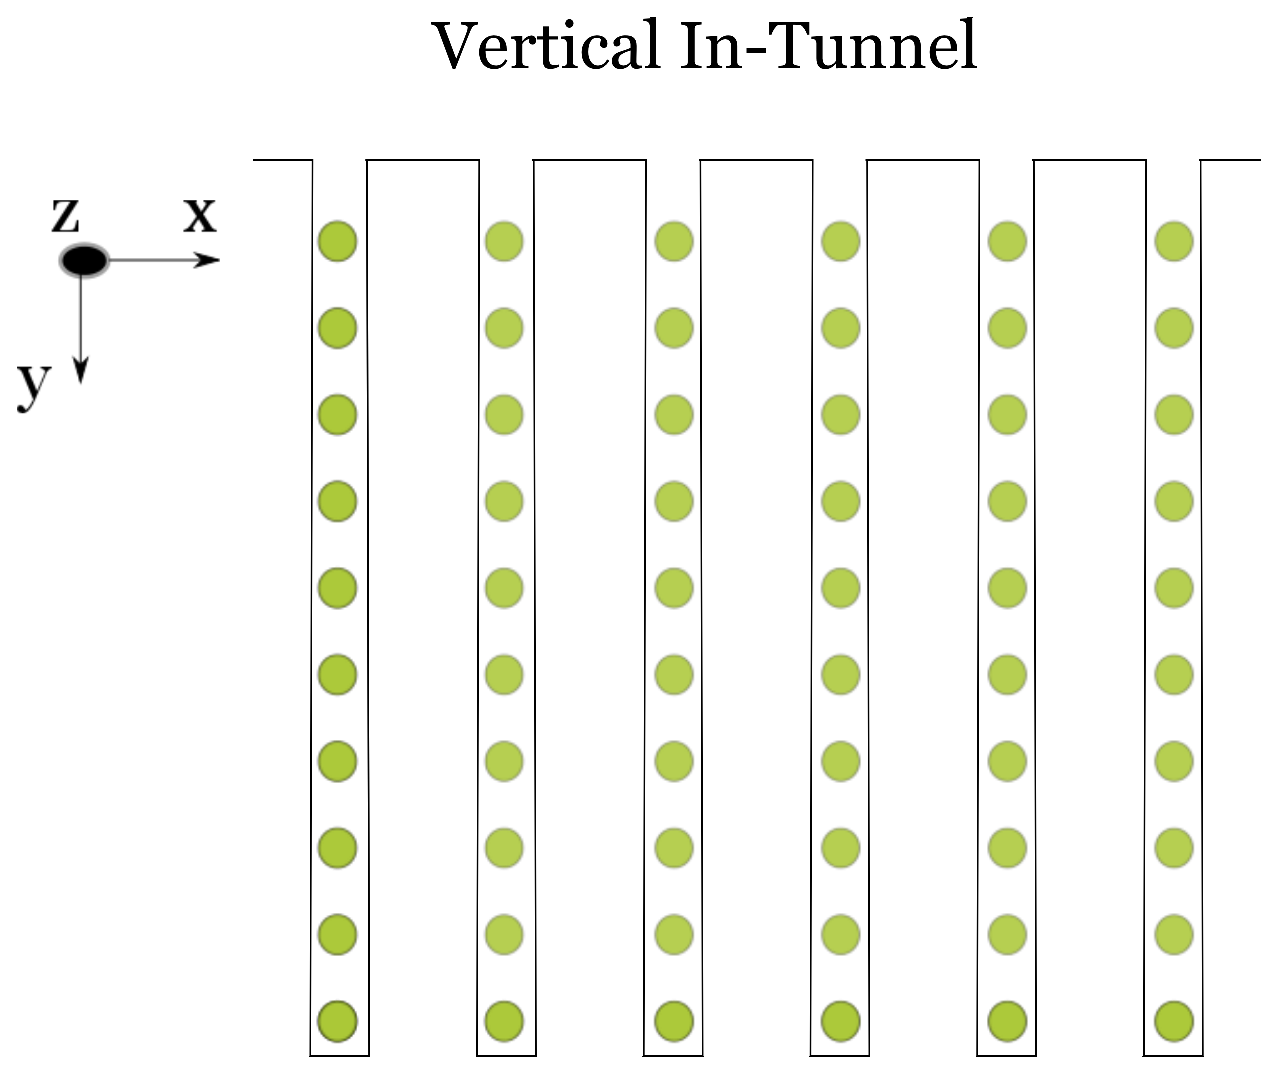
\includegraphics[width=0.75\textwidth]{vertical.eps}
    \end{figure}
  \end{minipage}
  \hspace{0.01cm}
  \begin{minipage}{0.49\textwidth}
    \begin{figure}[h!]
      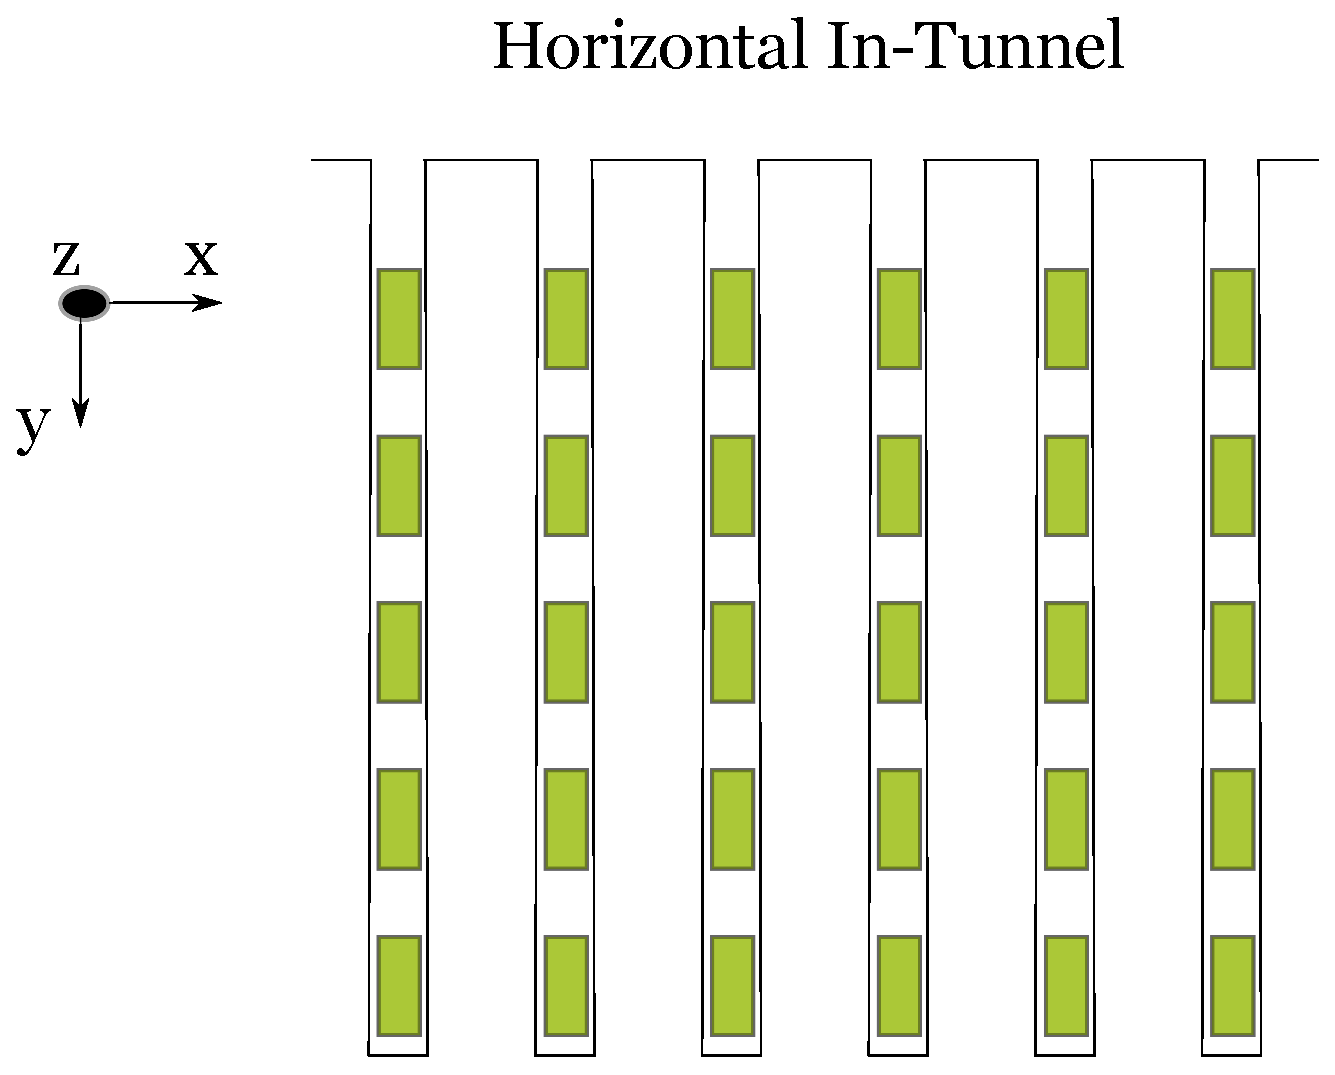
\includegraphics[width=0.8\textwidth]{horizontal.eps}
    \end{figure}
    \begin{figure}[h!]
      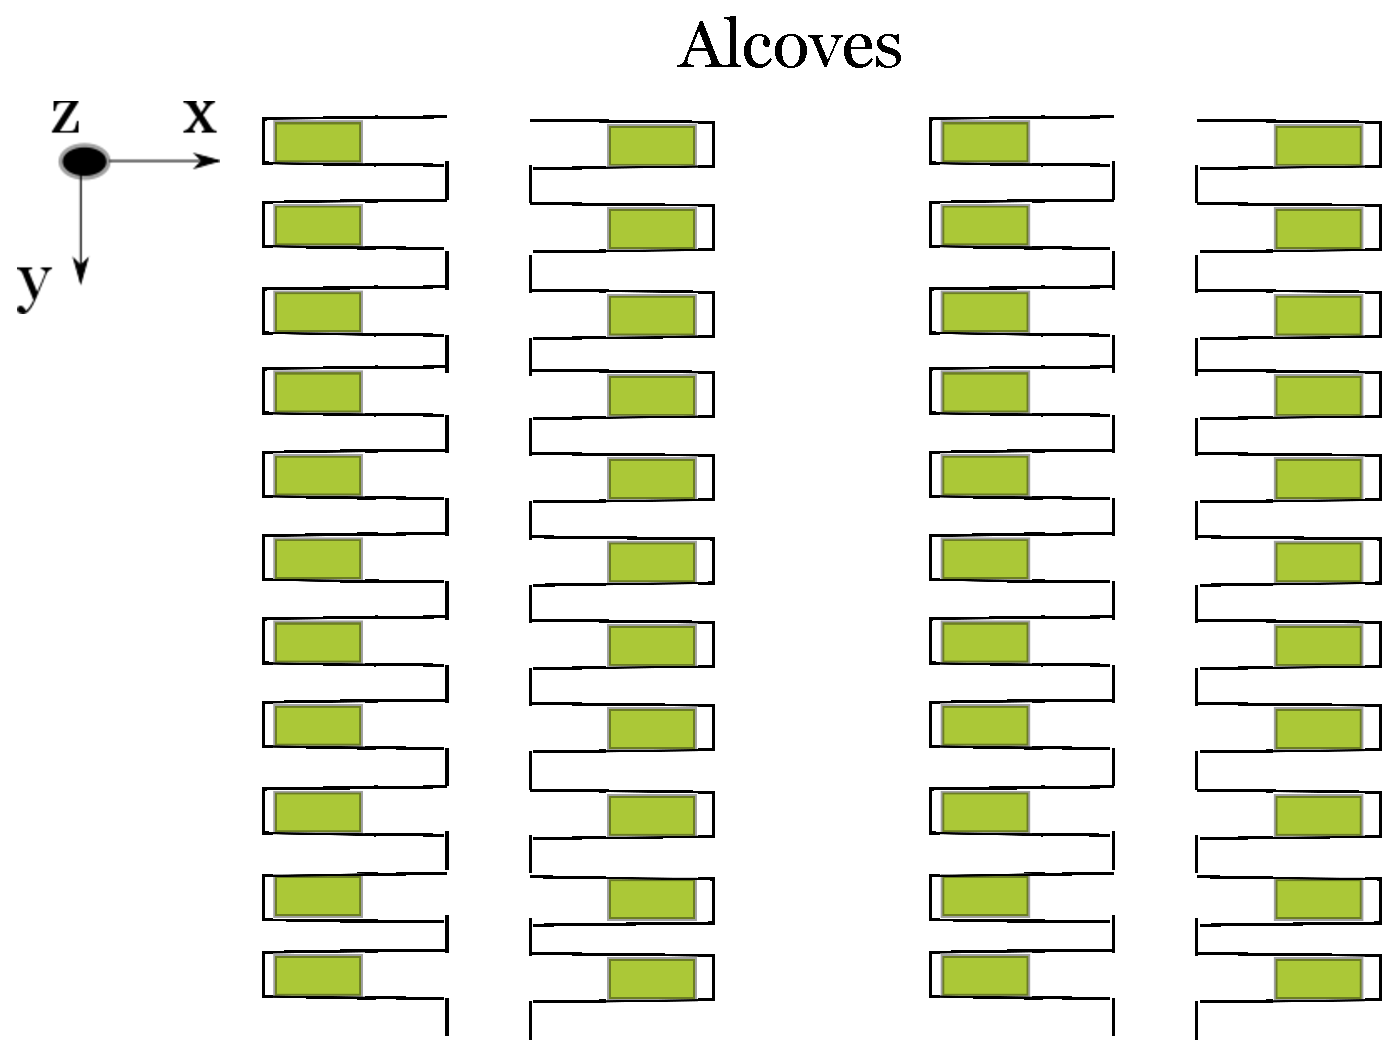
\includegraphics[width=0.8\textwidth]{alcoves.eps}
    \end{figure}
  \end{minipage}

\end{frame}

\begin{frame}
  \footnotesize{
  \frametitle{Unsaturated, Ventilated Concepts}
  \begin{figure}[htbp!]
  \begin{center}
    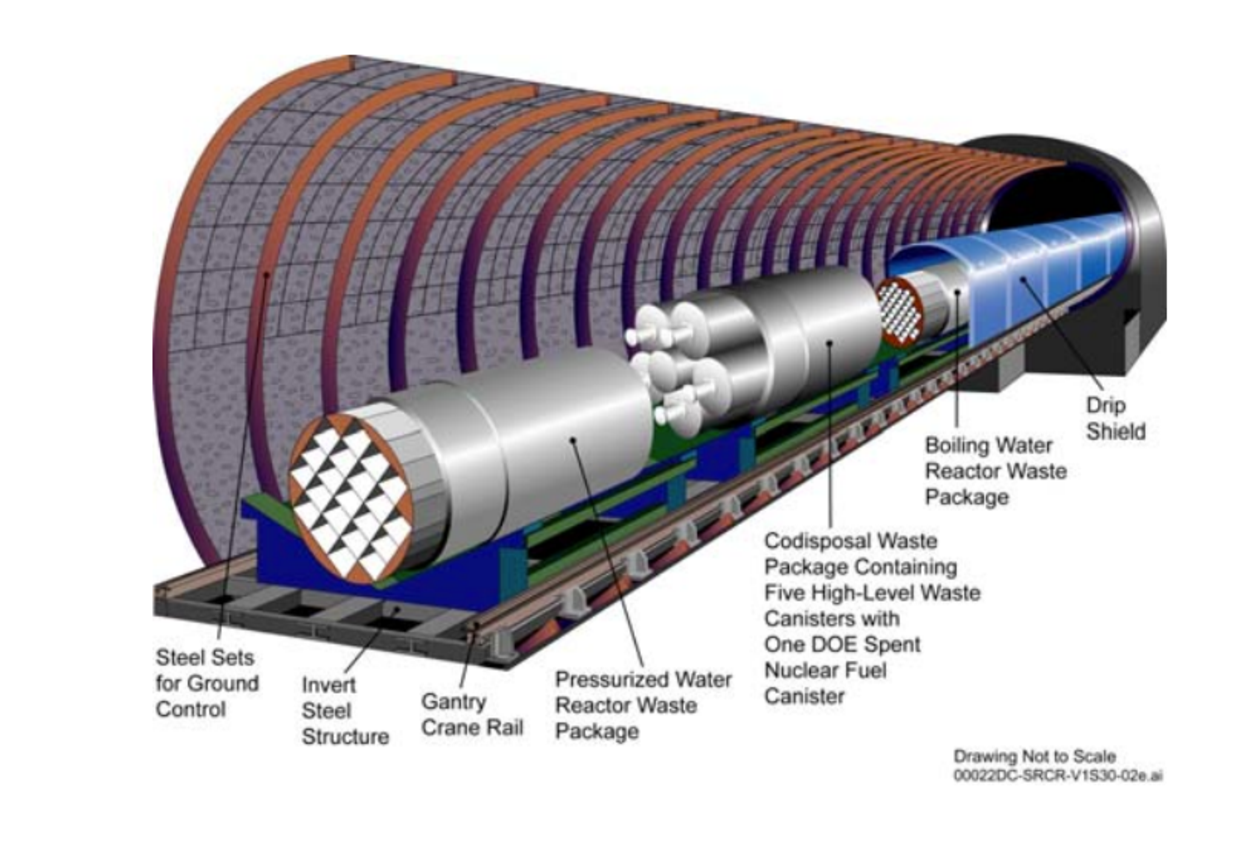
\includegraphics[height=0.7\textwidth]{yucca_tunnel.eps}
  \end{center}
  \caption{The current U.S. geologic disposal concept \cite{peters_whats_2013}.}
  \label{fig:yucca_tunnel}
\end{figure}

}
\end{frame}

\begin{frame}
  \footnotesize{
  \frametitle{Saturated , Enclosed Concepts} 
 \begin{figure}[h!]
    \begin{center}
      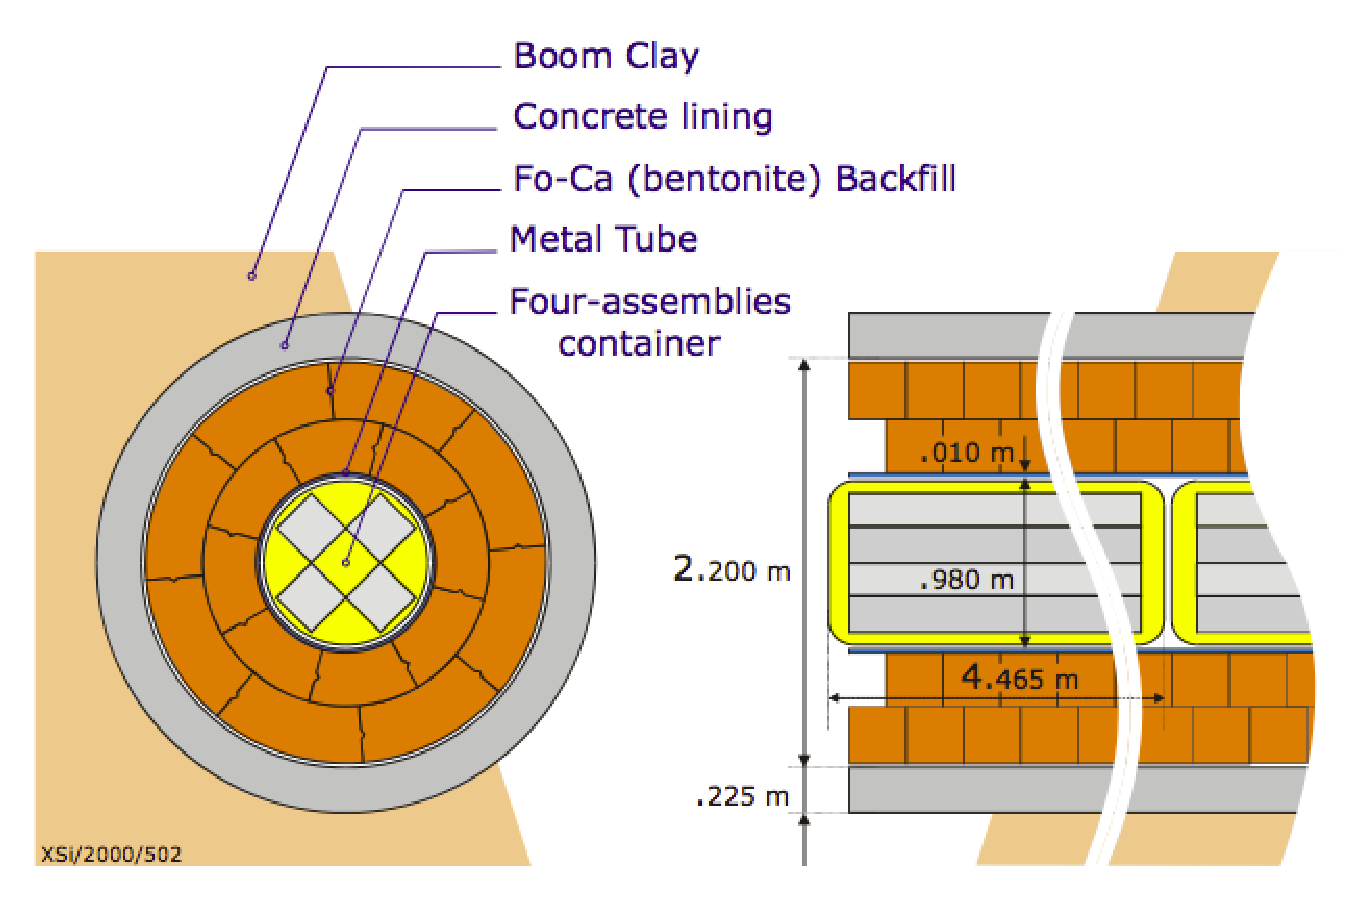
\includegraphics[height=.7\textheight]{belgianClayRedImp.eps}
    \end{center}
    \caption{The Belgian reference concept in Boom Clay is backfilled very soon
   after waste emplacement without a ventilation period and is located below the water table
   \cite{von_lensa_red-impact_2008}.}
    \label{fig:belgianClayRedImp}
  \end{figure}
}
\end{frame}

\subsection{Geologies}


\begin{frame}[ctb!]
  \frametitle{Tuff (Yucca) Disposal Environments}
  \footnotesize{
    \begin{figure}[htbp!]
  \begin{center}
    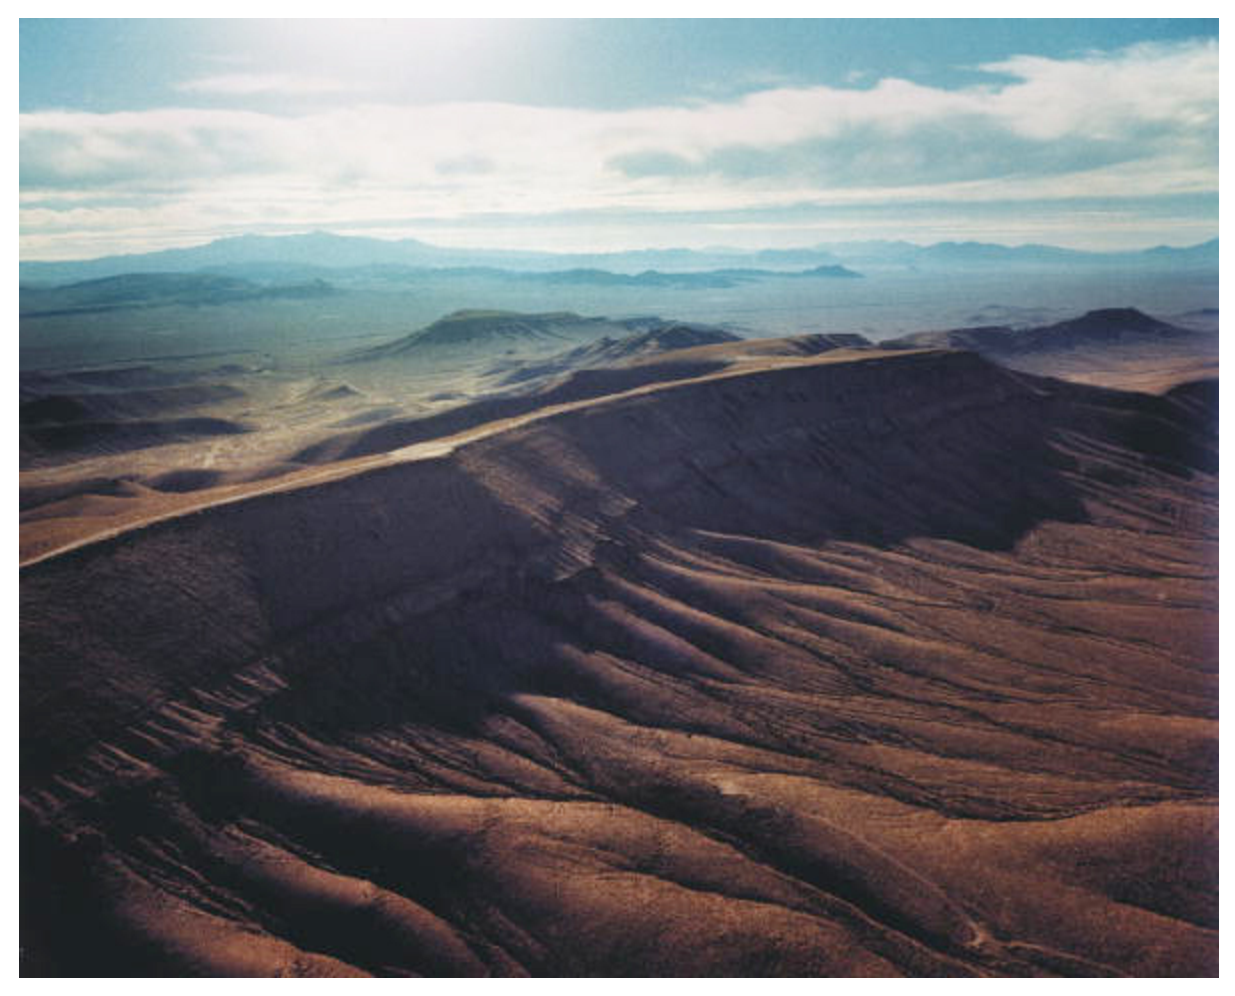
\includegraphics{yucca_site.eps}
  \end{center}
  \caption{Yucca Mountain in southern Nevada \cite{wherever_you_got_this}.}
  \label{fig:yucca_site}
\end{figure}

  }
\end{frame}

\begin{frame}[ctb!]
  \frametitle{Alternative Disposal Geology Options}
   \begin{minipage}{0.44\textwidth}
     \begin{figure}[h!]
         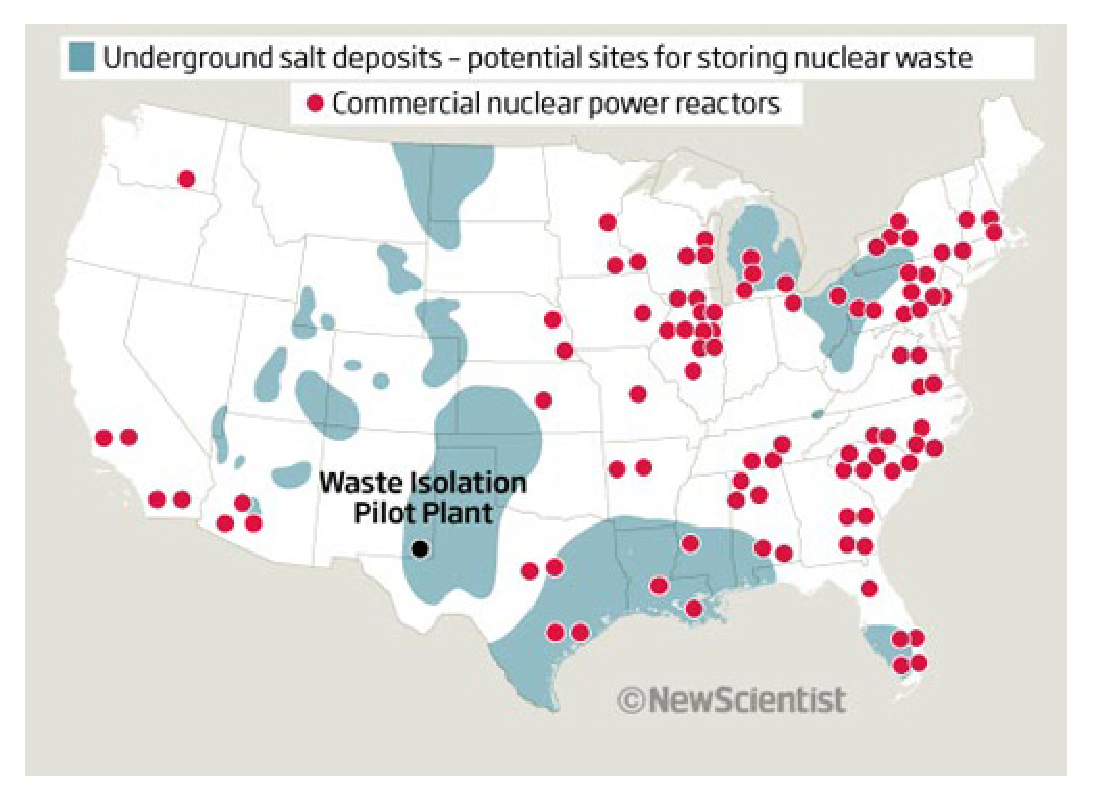
\includegraphics[width=0.8\textwidth]{saltNewScientist.eps}
         \caption{U.S. Salt Deposits, ref. \cite{newscientist_where_2011}.}
     \end{figure}
     \begin{figure}[h!]
         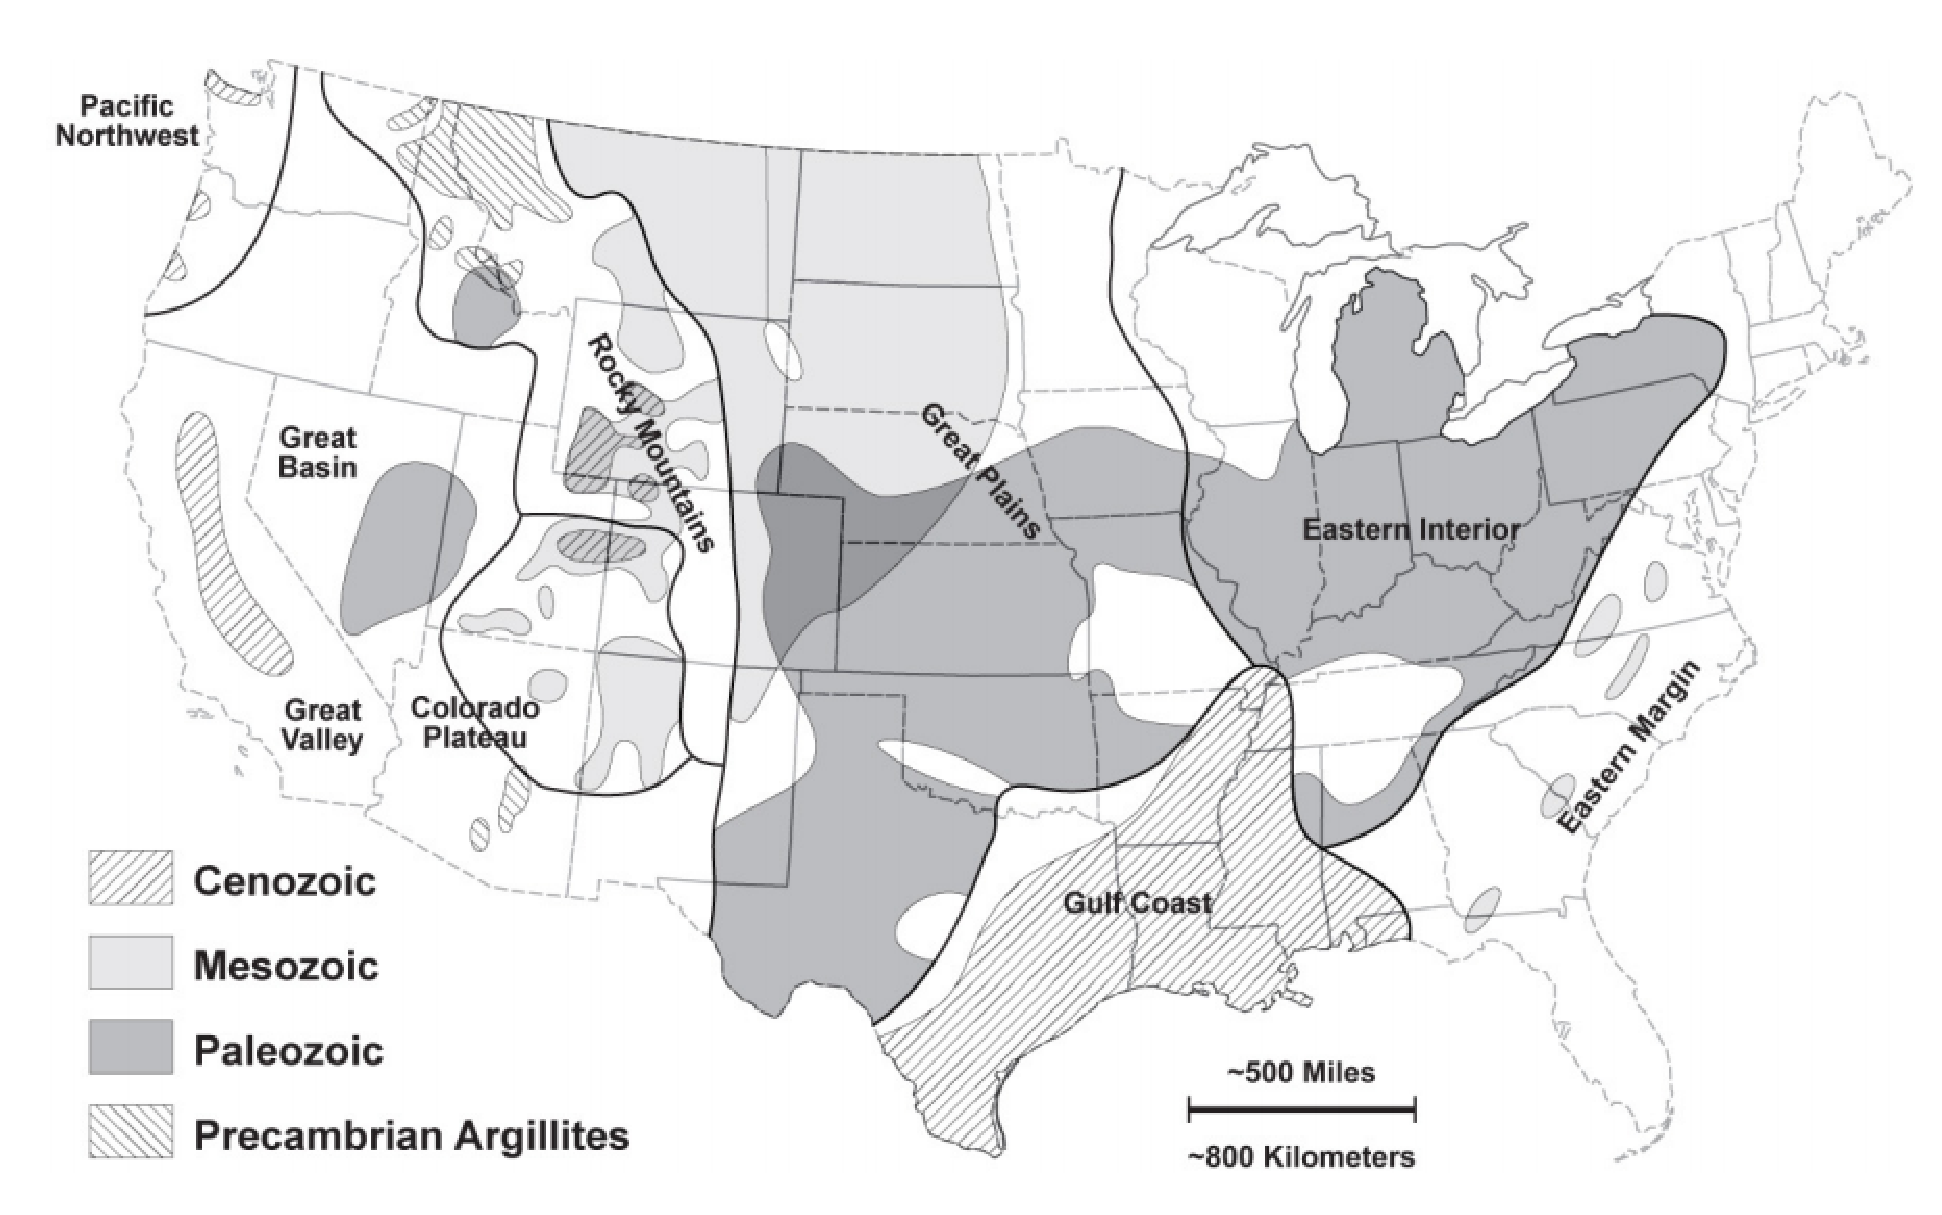
\includegraphics[width=0.8\textwidth]{clayGonzales.eps}
         \caption{U.S. Clay Deposits, ref. \cite{gonzales_shales_1985}.}
     \end{figure}
   \end{minipage}
   \hspace{0.01cm}
   \begin{minipage}{0.44\textwidth}
     \begin{figure}[h!]
         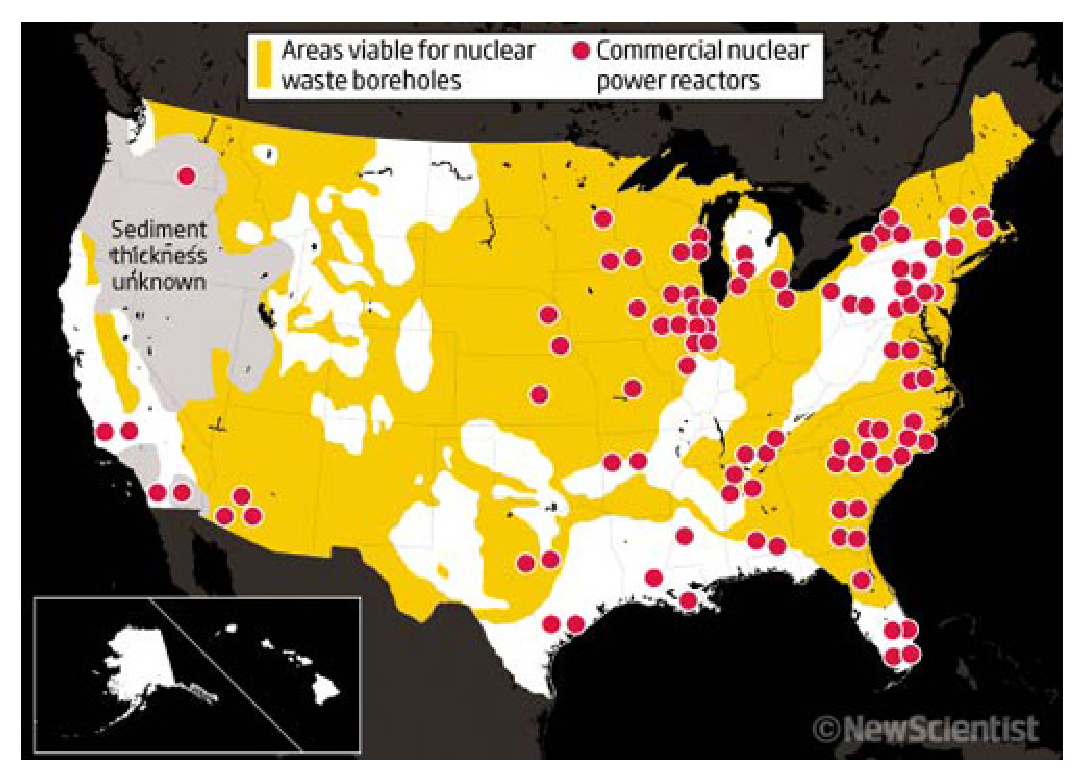
\includegraphics[width=0.8\textwidth]{boreholeNewScientist.eps}
         \caption{U.S. Crystalline Basement, ref.  \cite{newscientist_where_2011}.}
     \end{figure}
     \begin{figure}[h!]
         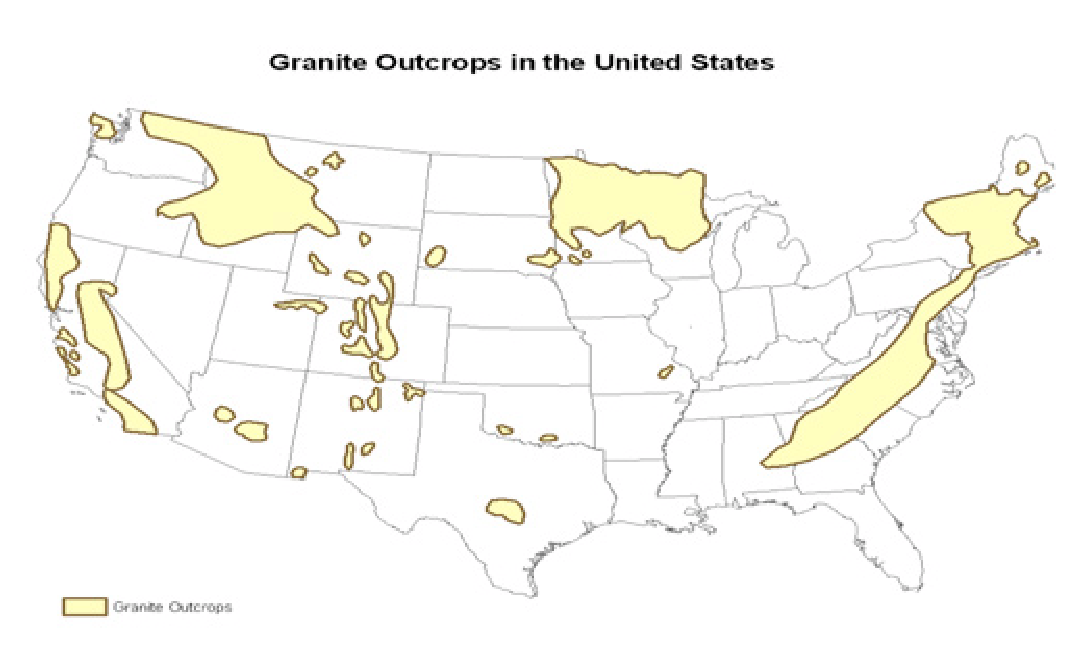
\includegraphics[width=0.8\textwidth]{graniteBush.eps}
         \caption{U.S. Granite Beds, ref. \cite{bush_economic_1976}.}
     \end{figure}
   \end{minipage}
\end{frame}

\begin{frame}[ctb!]
  \frametitle{Clay Disposal Environments}
  \footnotesize{

  \begin{figure}[h!]
    \begin{center}
      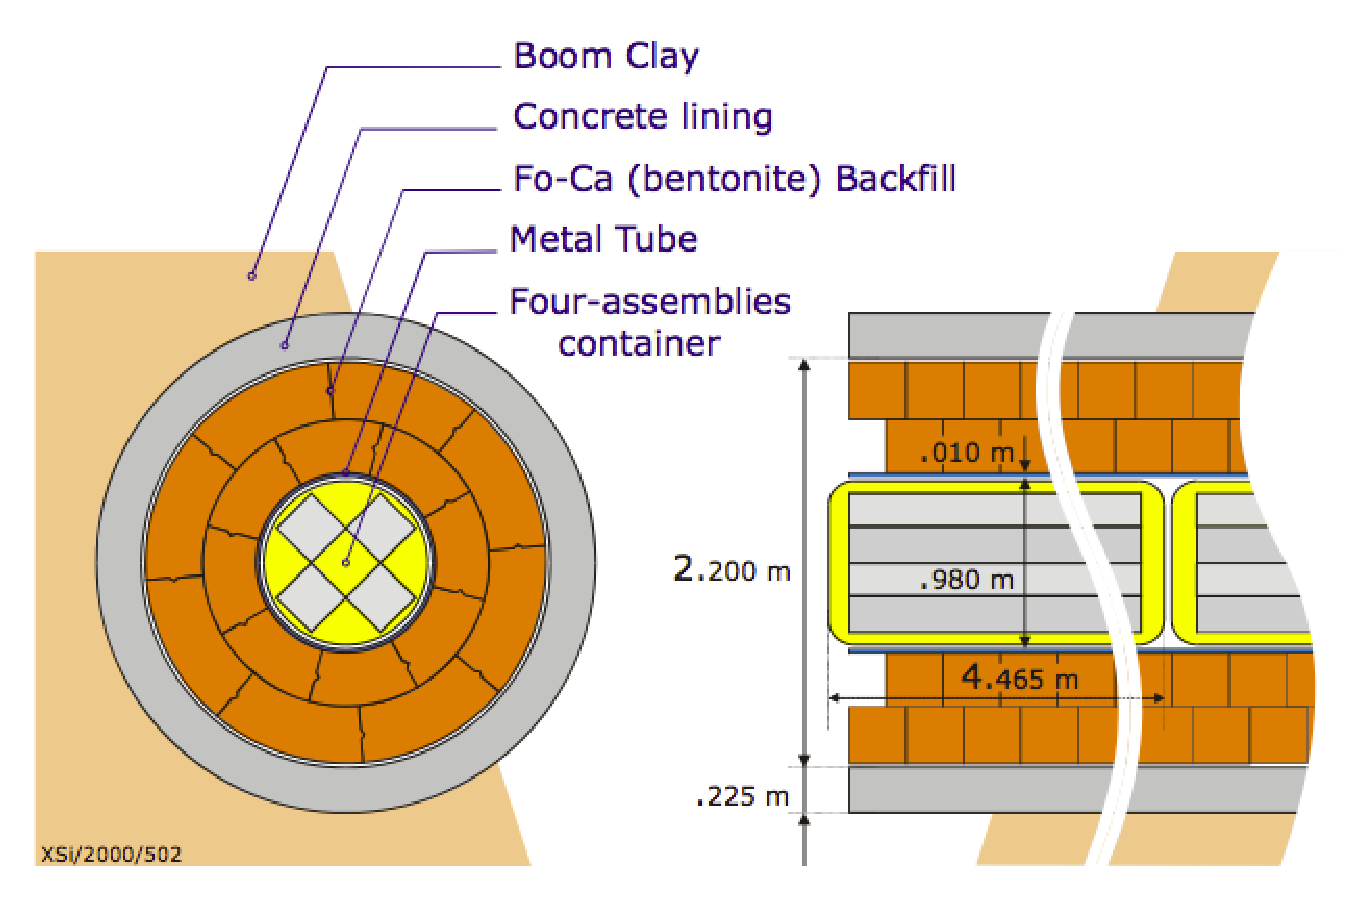
\includegraphics[height=.7\textheight]{belgianClayRedImp.eps}
    \end{center}
    \caption{Belgian reference concept in Boom Clay 
    \cite{von_lensa_red-impact_2008}.}
    \label{fig:belgianClayRedImp}
  \end{figure}

}
\end{frame}

\begin{frame}[ctb!]
  \frametitle{Granite Disposal Environments}
  \footnotesize{

  \begin{figure}[h!]
    \begin{center}
      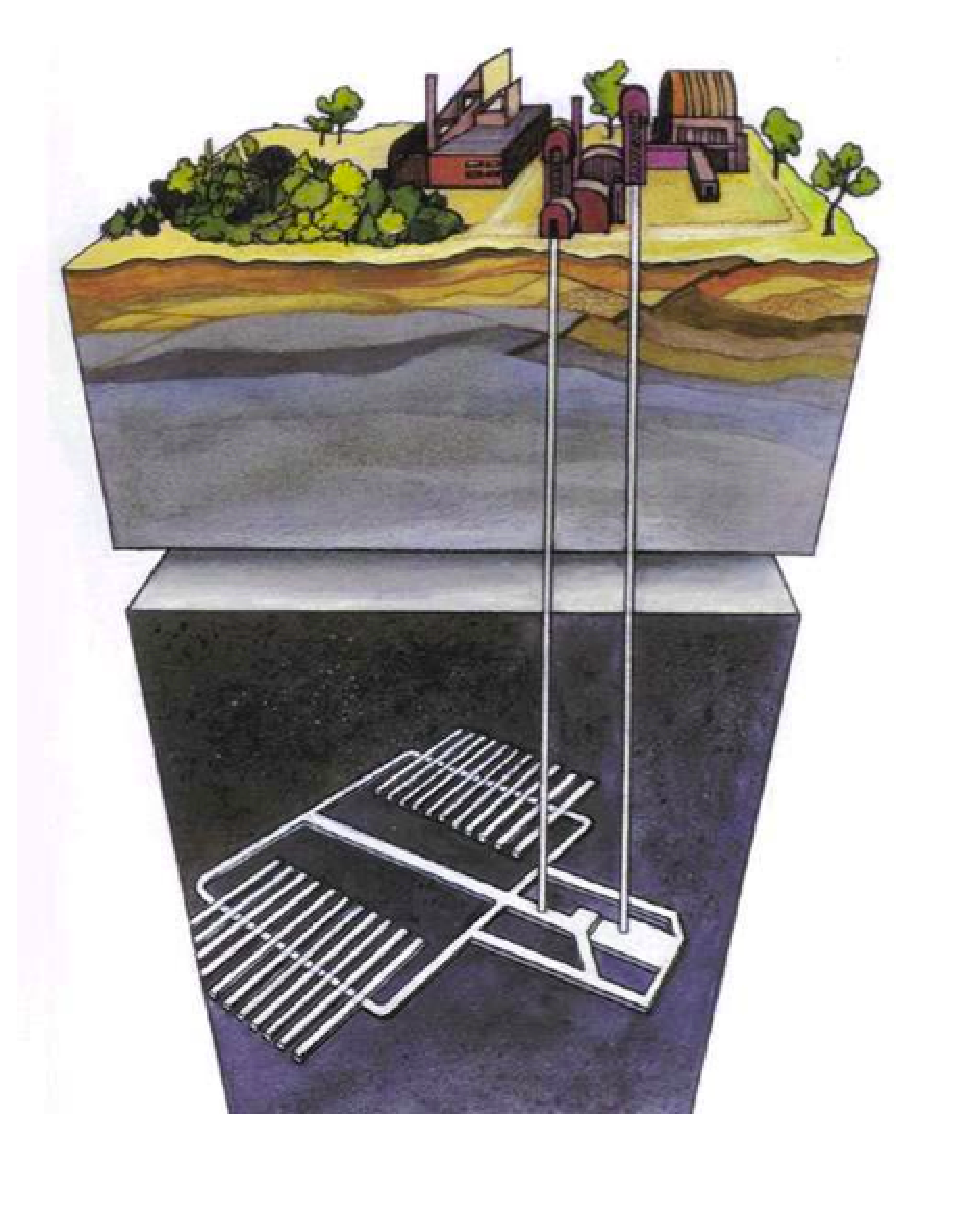
\includegraphics[height=.7\textheight]{czechGraniteRedImp.eps}
    \end{center}
    \caption{Czech reference concept in Granite 
    \cite{von_lensa_red-impact_2008}.}
    \label{fig:czechGraniteRedImp}
  \end{figure}
}
\end{frame}

\begin{frame}[ctb!]
  \frametitle{Salt Disposal Environments}
  \footnotesize{

  \begin{figure}[h!]
    \begin{center}
      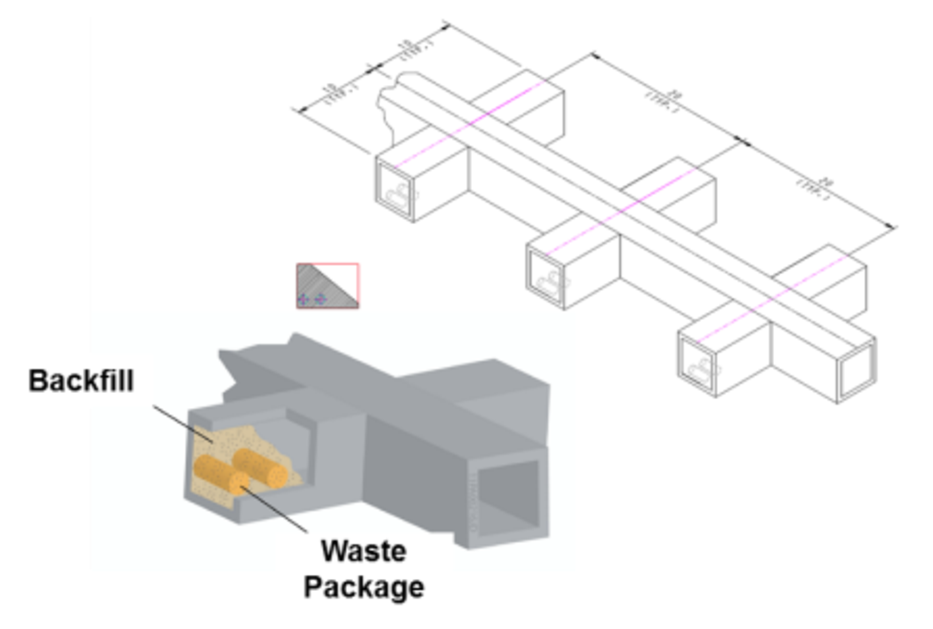
\includegraphics[height=.7\textheight]{carter_salt_layout.eps}
    \end{center}
    \caption{DOE-NE Used Fuel Disposition Campaign  concept in 
    Salt \cite{hardin_generic_2011}.}
    \label{fig:salt_layout}
  \end{figure}
}
\end{frame}
\begin{frame}[ctb!]
  \frametitle{Salt Disposal Environments}
  \footnotesize{

  \begin{figure}[h!]
    \begin{center}
      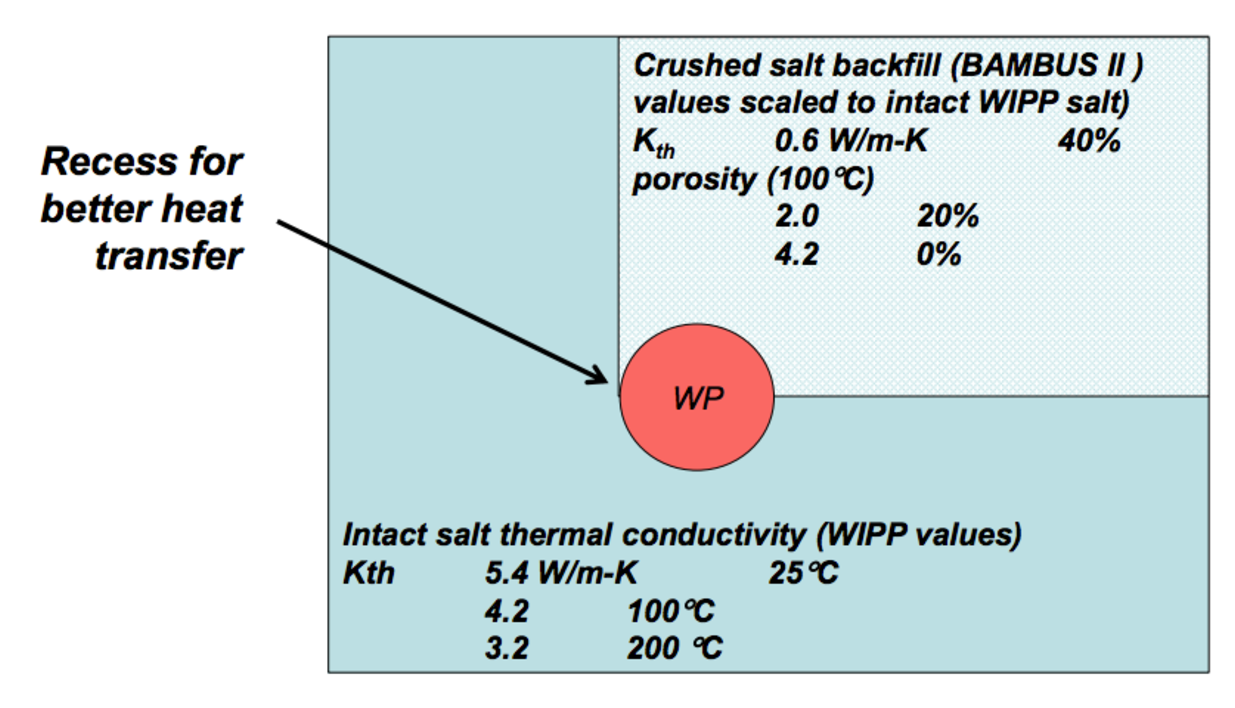
\includegraphics[height=.7\textheight]{hardin_salt_layout.eps}
    \end{center}
    \caption{DOE-NE Used Fuel Disposition Campaign  concept in 
    Salt \cite{harder_generic_2011}.}
    \label{fig:hardin_salt_layout}
  \end{figure}
}
\end{frame}

\begin{frame}[ctb!]
  \frametitle{Deep Borehole Disposal Environment}
  \footnotesize{

  \begin{figure}[h!]
    \begin{center}
      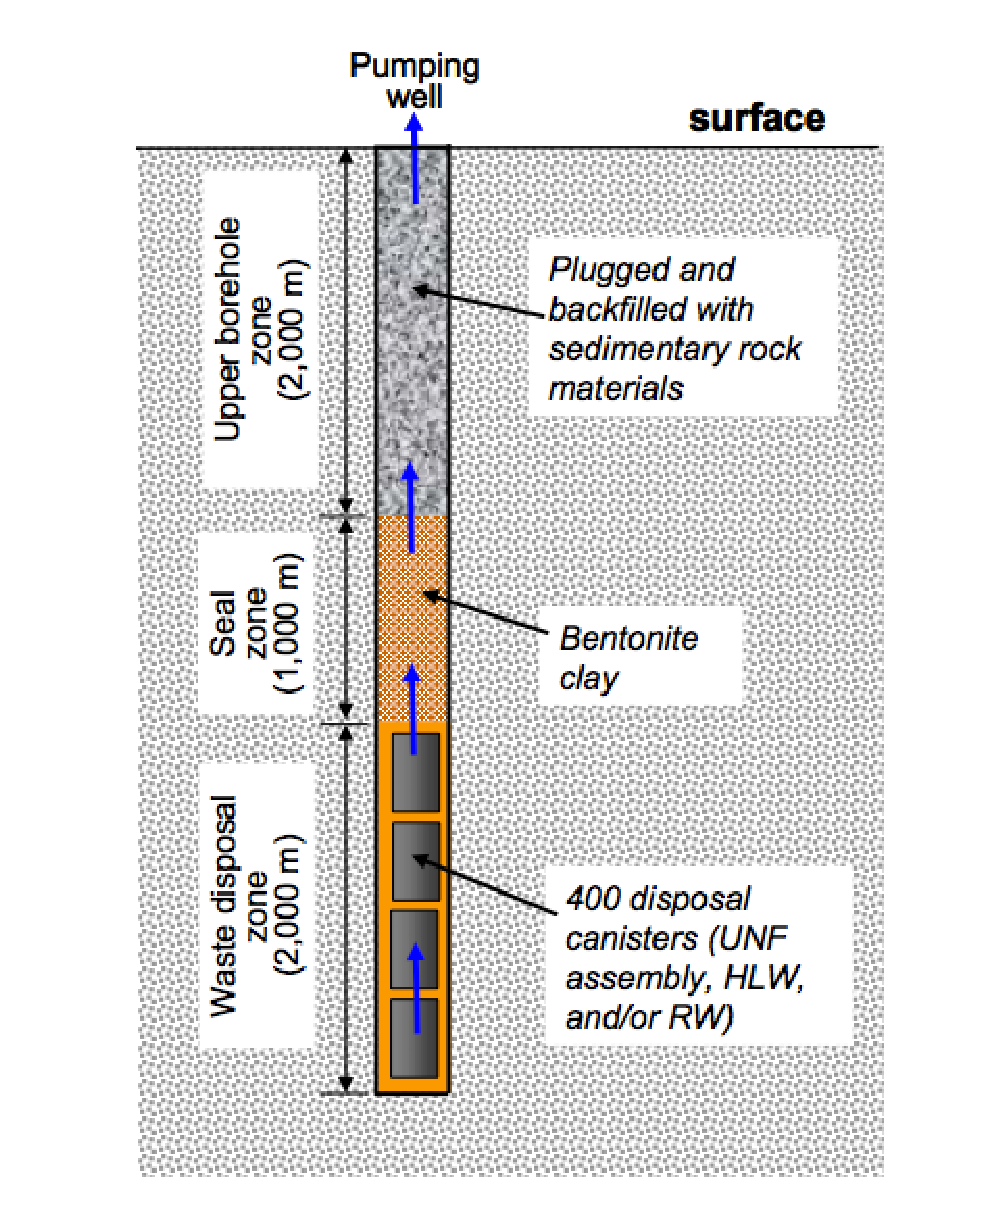
\includegraphics[height=.7\textheight]{boreholeGPAM.eps}
    \end{center}
    \caption{DOE-NE Used Fuel Disposition Campaign Deep Borehole concept 
    \cite{clayton_generic_2011}.}
    \label{fig:boreholeGPAM}
  \end{figure}
}
\end{frame}




\section{Geologic Repository Performance}
\subsection{Metrics}

%%----------------------------------------%%
\begin{frame}[ctb!]
\footnotesize{
  \frametitle{<++>}
  <++>
}
\end{frame}

%%----------------------------------------%%
\begin{frame}[ctb!]
\footnotesize{
  \frametitle{<++>}
  <++>
}
\end{frame}

\subsection{Thermal Loading}

%%----------------------------------------%%
\begin{frame}[ctb!]
\footnotesize{
  \frametitle{<++>}
  <++>
}
\end{frame}

%%----------------------------------------%%
\begin{frame}[ctb!]
\footnotesize{
  \frametitle{<++>}
  <++>
}
\end{frame}

\subsection{Radionuclide Transport and Release}

%%----------------------------------------%%
\begin{frame}[ctb!]
  \frametitle{Release Mechanisms}
  \begin{itemize} 
  \item Human Disruption
  \item Natural Disruption
  \item Barrier Dissolution
  \item Advection
  \item Diffusion
  \item Sorption
  \item Solubility Limitation
  \item ... 
  \end{itemize}
\end{frame}

%%----------------------------------------%%
\begin{frame}
\frametitle{Solubility Sensitivity In A Clay Model}
\begin{figure}[ht]
  \centering
  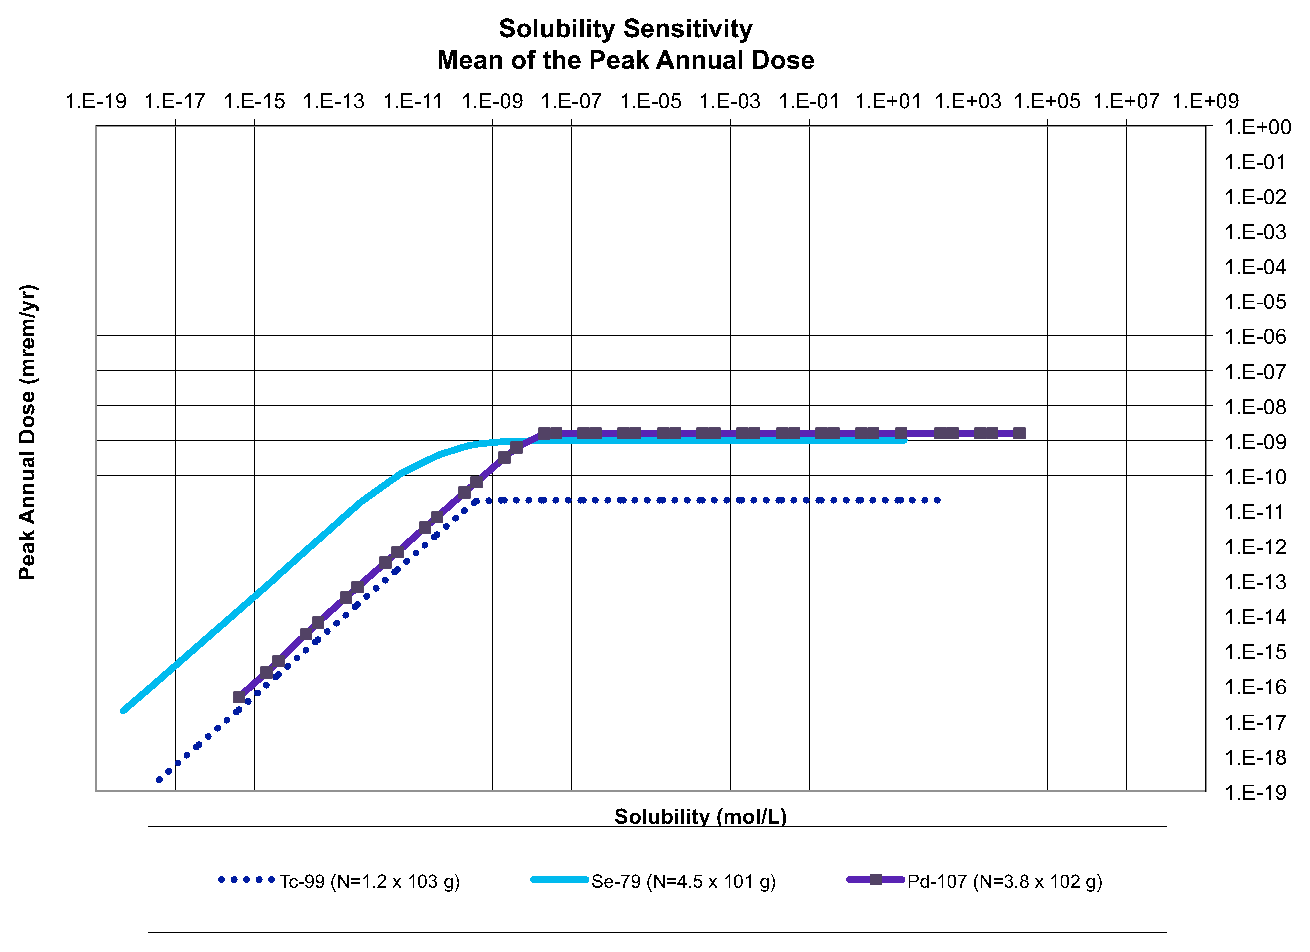
\includegraphics[width=0.7\linewidth]{Solubility_Summary.eps}
  \caption{Solubility limit sensitivity. The peak annual dose due to an 
  inventory, $N$, of each isotope.}
  \label{fig:SolSum}
\end{figure}
\end{frame}

%%----------------------------------------%%
\begin{frame}[ctb]
\frametitle{Retardation Sensitivity In A Clay Model}
\begin{figure}[ht]
  \centering
  \includegraphics[width=0.7\linewidth]{Partitioning_Summary.eps}
  \caption{$K_d$ sensitivity.  The peak annual dose due to an inventory, 
  $N$, of each isotope.}
  \label{fig:KdSum}
\end{figure}
\end{frame}

%%----------------------------------------%%
\begin{frame}[c]
  \frametitle{Example : Vertical Advective Velocity and Diffusion Coefficient}
\begin{figure}[htp!]
\centering
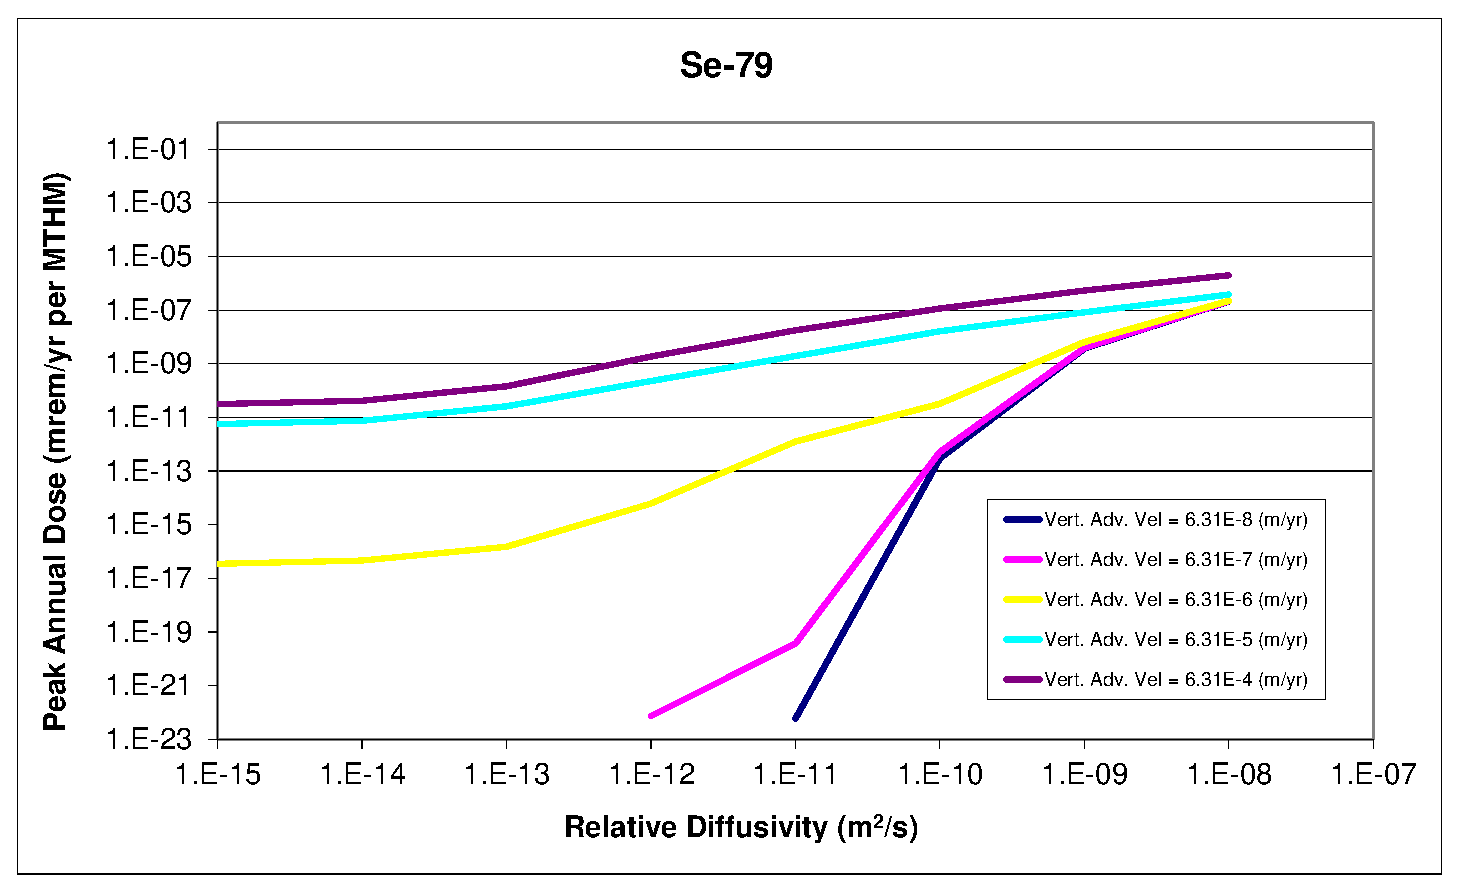
\includegraphics[width=0.8\textwidth]{Se-79.eps}
\caption{$^{79}Se$.  $Se$ is non sorbing, but solubility limited in clay.  For low vertical advective velocity, the system is diffusion dominated.}
\label{fig:VAdvVelSe79}
\end{figure}
\end{frame}

%%----------------------------------------%%
\begin{frame}[c]
  \frametitle{Example : Vertical Advective Velocity and Diffusion Coefficient}
\begin{figure}[ht!]
\centering
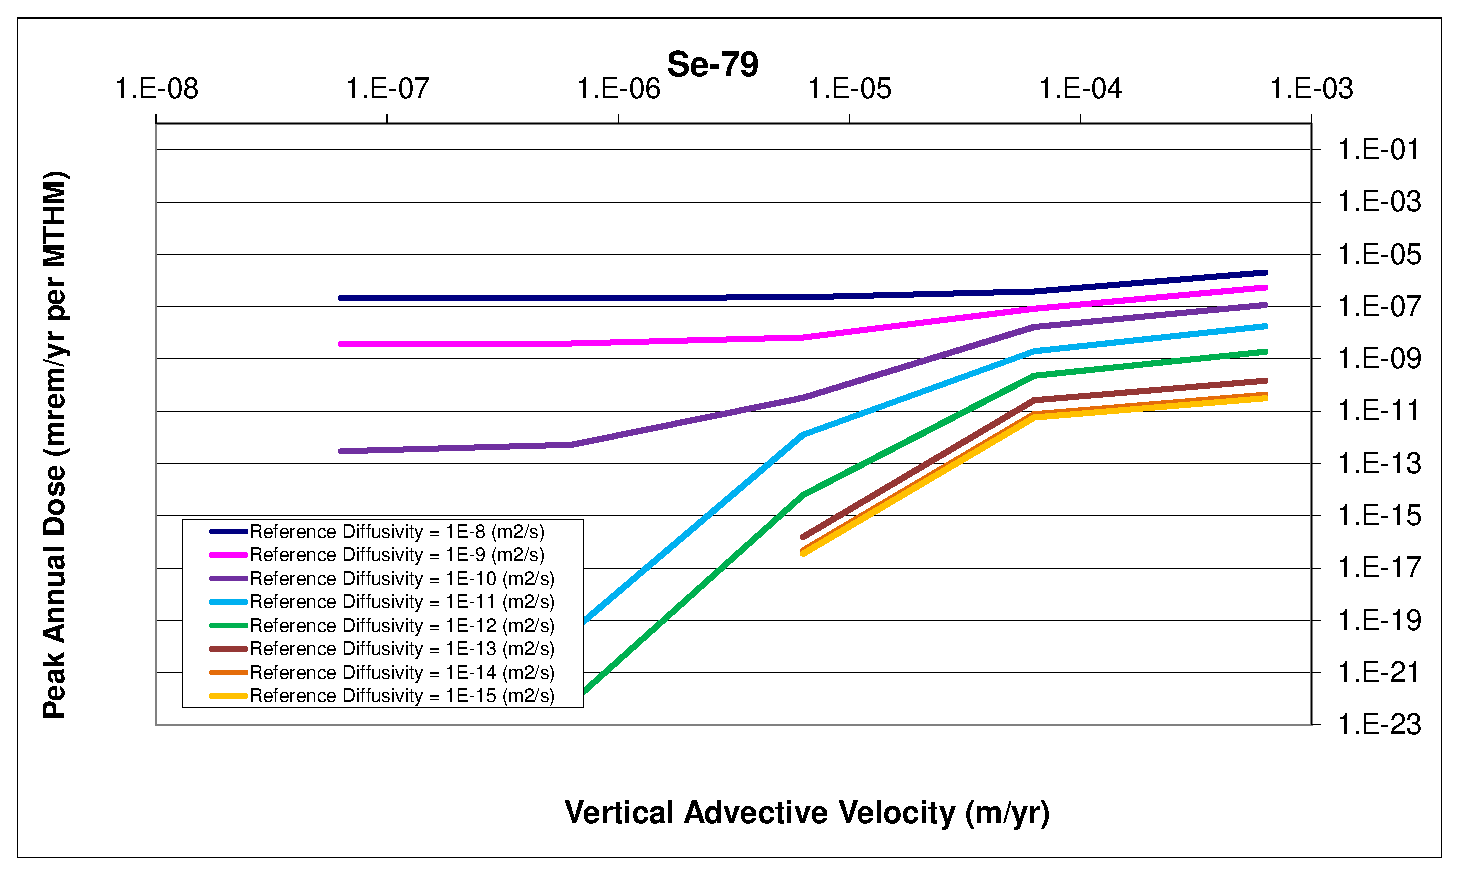
\includegraphics[width=0.8\textwidth]{Se-79-VAdvVel.eps}
\caption{$^{79}Se$.
$Se$ is non sorbing, but solubility limited in clay.
For high vertical advective 
velocity, the diffusivity remains important even in the advective regime as 
spreading facilitates transport in the presence of solubility limited 
transport.} 
\label{fig:VAdvVelSe79VAdvVel}
\end{figure}
\end{frame}



\section{Fuel Cycle Impacts}
\subsection{Thermal Contributors}

%%----------------------------------------%%
\begin{frame}[ctb!]
  \frametitle{Heat Contributors In PWR SNF}
\footnotesize{
  \begin{figure}[htbp!]
  \begin{center}
    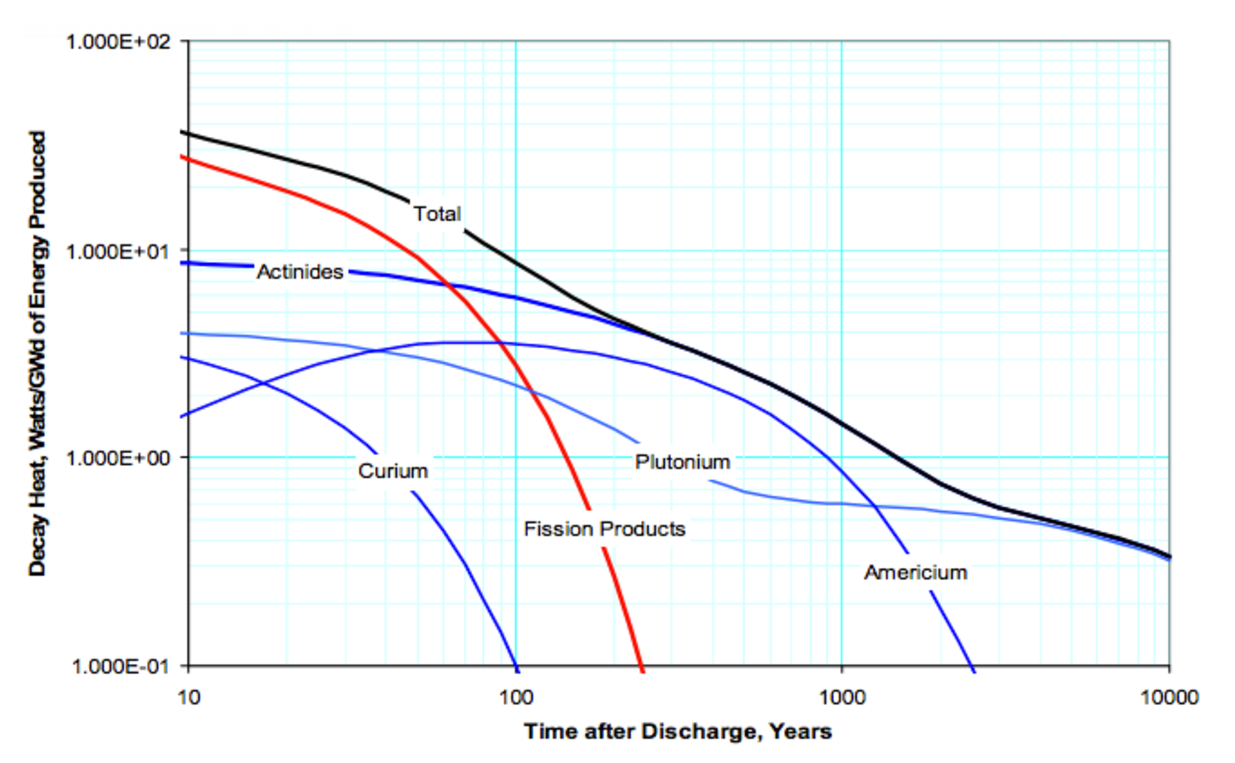
\includegraphics[width=0.7\textheight]{wigeland_heat.eps}
  \end{center}
  \caption{Heat contributors in a canonical PWR 
    fuel\cite{wigeland_relationship_2010}.}
  \label{fig:<++>}
\end{figure}

}
\end{frame}

%%----------------------------------------%%
\begin{frame}[ctb!]
  \frametitle{Heat Contributors in PWR SNF}
\footnotesize{
  \begin{figure}[htbp!]
  \begin{center}
    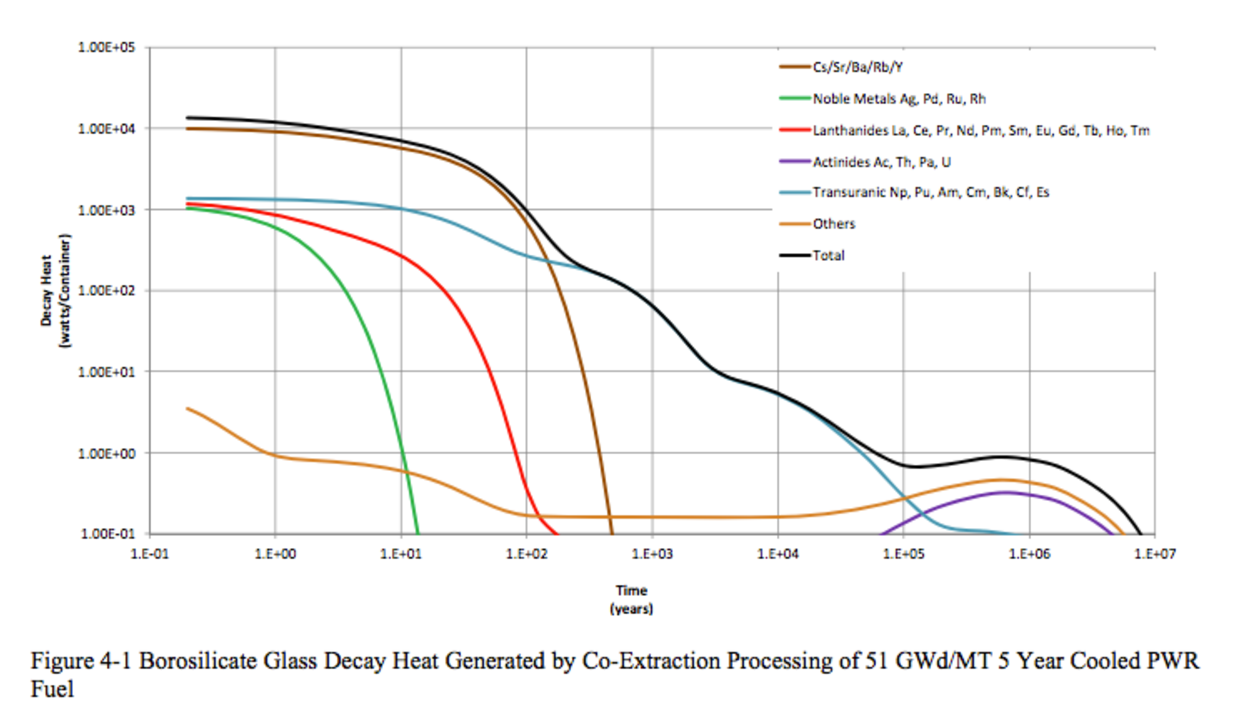
\includegraphics[width=0.7\textheight]{carter_coex_heat.eps}
  \end{center}
  \caption{Heat contributors in the primary result of a once through PWR fuel 
    cycle \cite{carter_us_2011}.}
  \label{fig:carter_coex_heat}
\end{figure}

}
\end{frame}
%%----------------------------------------%%
\begin{frame}[ctb!]
  \frametitle{Heat Contributors in LWR Recycled MOX}
\footnotesize{
  \begin{figure}[htbp!]
  \begin{center}
    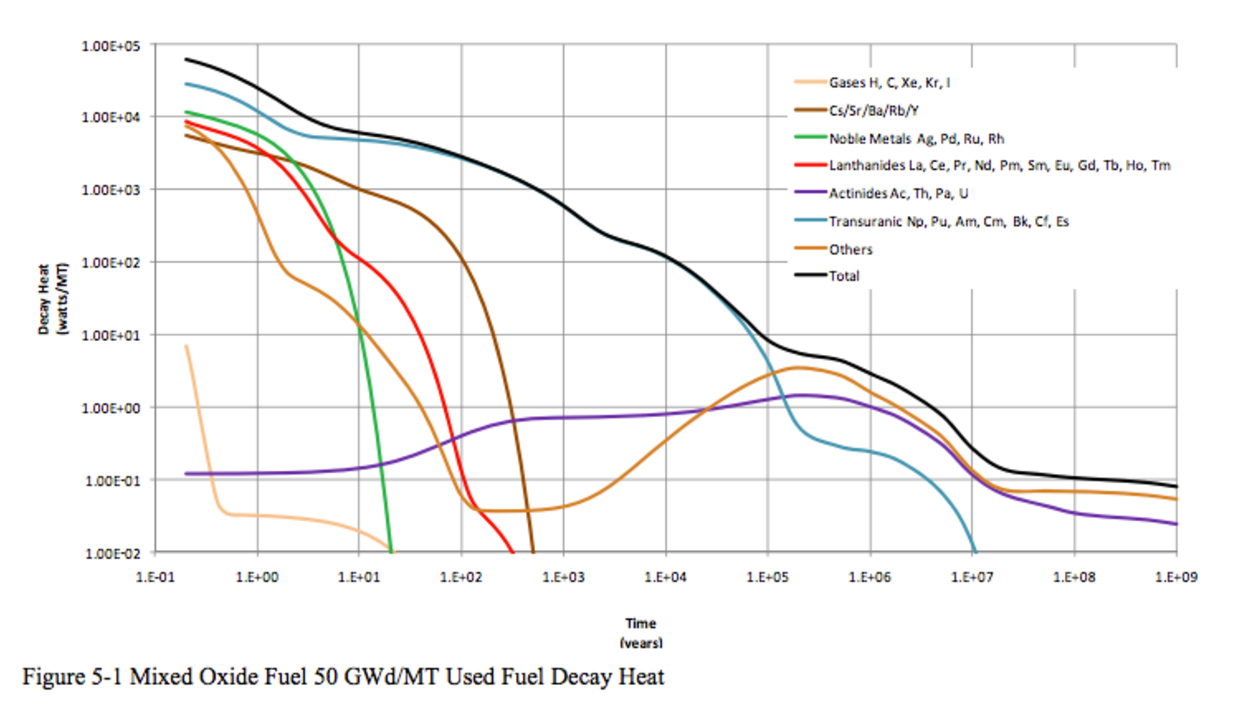
\includegraphics[width=0.7\textwidth]{carter_lwr_mox_heat.eps}
  \end{center}
  \caption{Heat contributors in the primary result of MOX recycling in an LWR
    \cite{carter_us_2011}.}
  \label{fig:carter_lwr_mox_heat}
\end{figure}

}
\end{frame}
%%----------------------------------------%%
\begin{frame}[ctb!]
  \frametitle{Heat Contributors After NUEX Recycling}
\footnotesize{
  \begin{figure}[htbp!]
  \begin{center}
    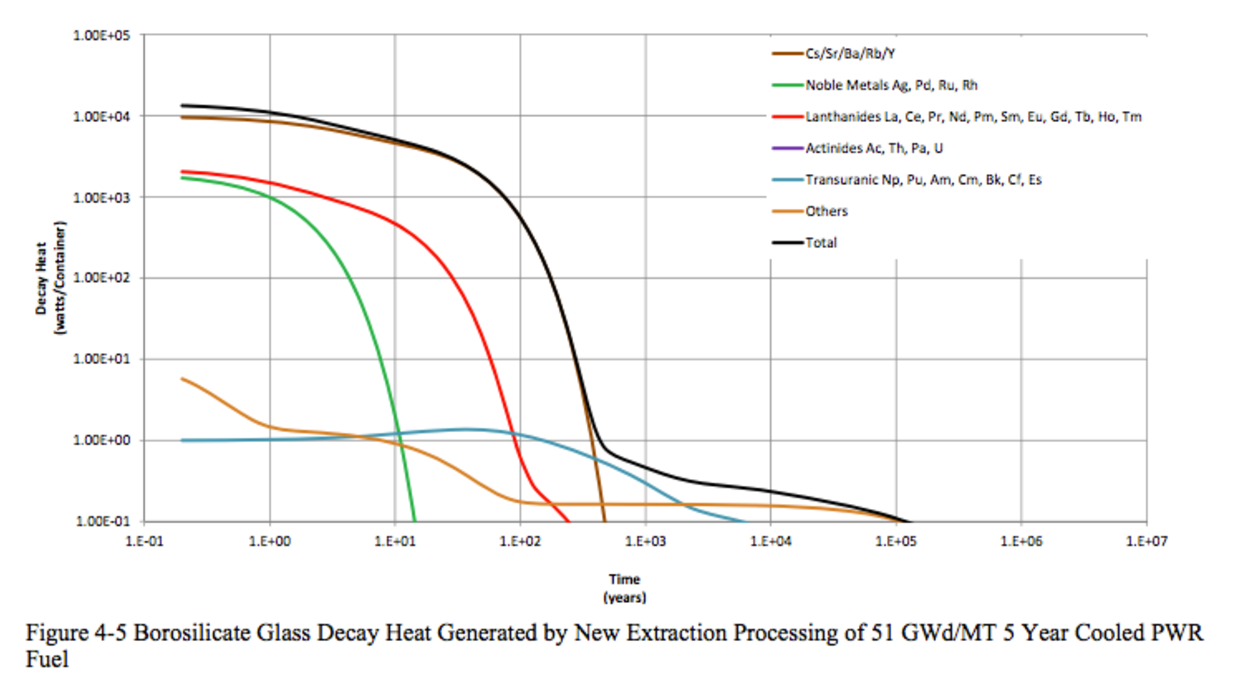
\includegraphics[width=0.7\textheight]{carter_nuex_heat.eps}
  \end{center}
  \caption{Heat contributors in the primary result of the NUEX extraction 
    process\cite{carter_us_2011}.}
  \label{fig:carter_nuex_heat}
\end{figure}

}
\end{frame}

%%----------------------------------------%%
\begin{frame}[ctb!]
  \frametitle{Heat Contributors After COEX Recycling}
\footnotesize{
  \begin{figure}[htbp!]
  \begin{center}
    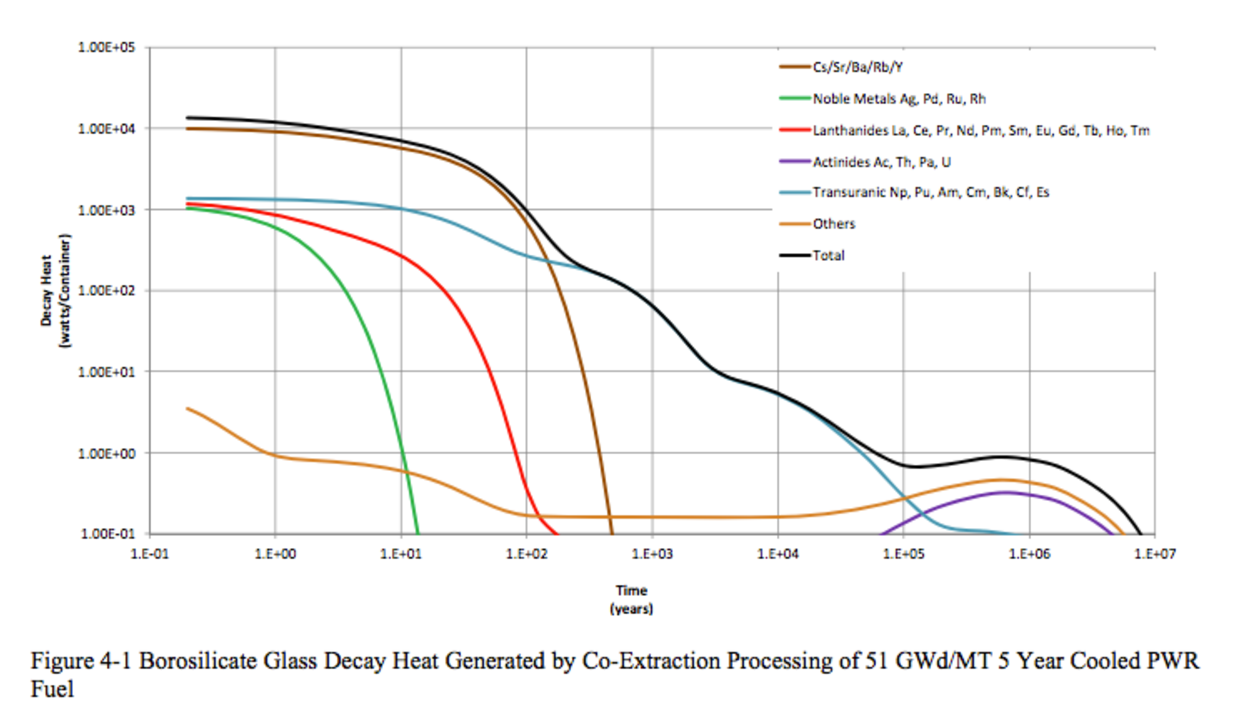
\includegraphics[width=0.7\textheight]{carter_coex_heat.eps}
  \end{center}
  \caption{Heat contributors in the primary result of the COEX extraction 
    process\cite{carter_us_2011}.}
  \label{fig:carter_coex_heat}
\end{figure}

}
\end{frame}
%%----------------------------------------%%
\begin{frame}[ctb!]
  \frametitle{Summary: Heat Contributing Isotopes in Various Fuel Cycles}
\footnotesize{
Dominant thermal contributors vary among fuel cycles. 
\begin{itemize}
   \item Recycling schemes are likely to reduce transuranics and actinides.
   \item Fission products such as Cs and Sr are powerful heat contributors in the first 1000 years, when capacity limiting peak heat is likely to occur in most geologies.
   \item Transuranics, Pu, Np, Am, and Cm are dominant long term heat contributors. Some extraction processes are more successful at removing those from the waste stream. 
\end{itemize}
}
\end{frame}

\subsection{Dose Contributors}

%%----------------------------------------%%
\begin{frame}[ctb!]
  \frametitle{Dose Contributors, PWR SNF In Yucca}
\footnotesize{
  \begin{figure}[htbp!]
  \begin{center}
    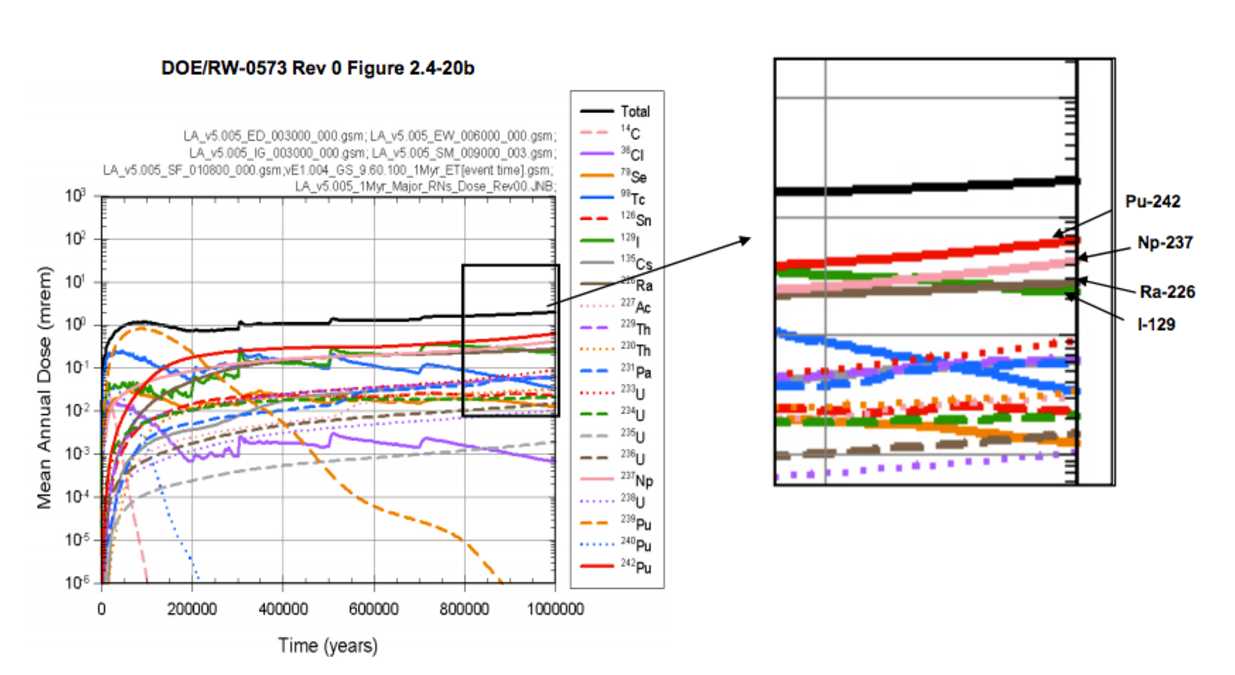
\includegraphics[width=0.7\textheight]{swift_dose_yucca.eps}
  \end{center}
  \caption{Dose contributors expected in the Yucca Mountain repository 
    \cite{swift_applying_2010}.}
  \label{fig:swift_dose_yucca}
\end{figure}

}
\end{frame}

%%----------------------------------------%%
\begin{frame}[ctb!]
  \frametitle{Dose Contributors, PWR SNF In Yucca}
\footnotesize{
  \begin{figure}[htbp!]
  \begin{center}
    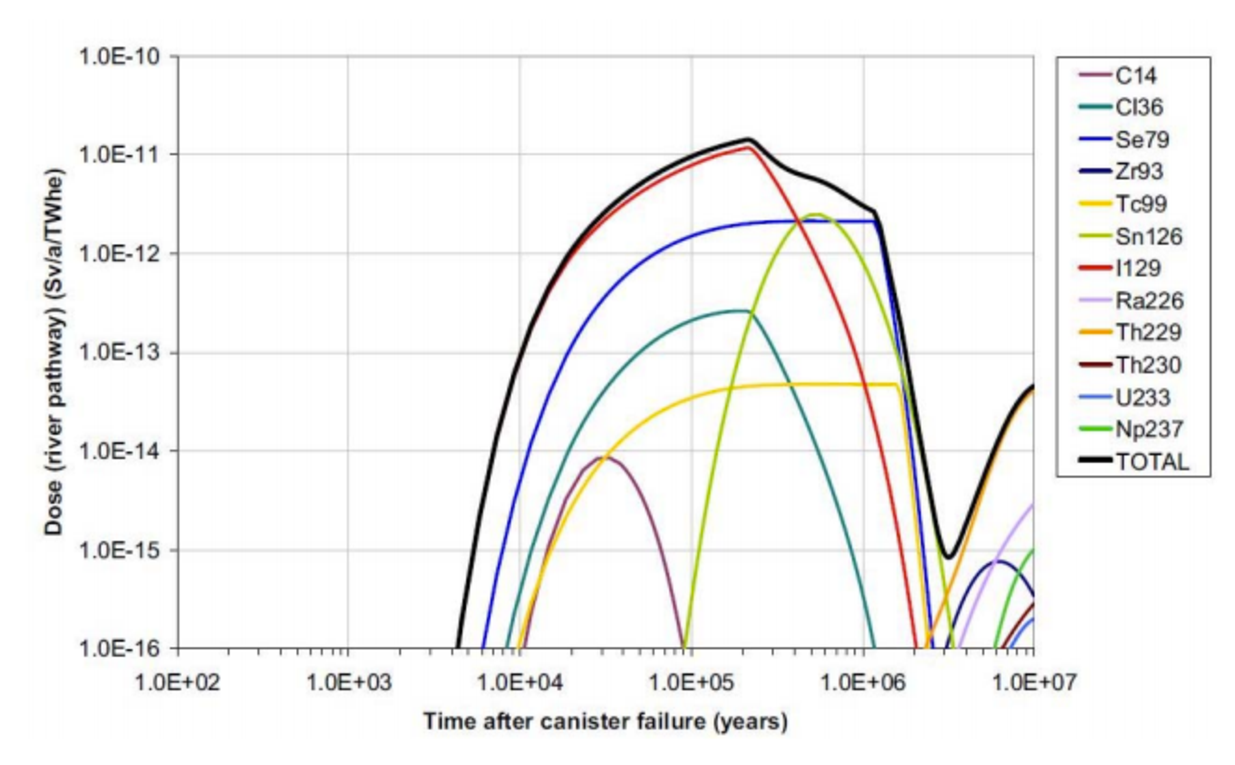
\includegraphics[width=0.7\textwidth]{wigeland_dose.eps}
  \end{center}
  \caption{Dose expected in Yucca Mountain by isotopic groups 
    \cite{wigeland_relationship_2010}.}
  \label{fig:wigeland_dose}
\end{figure}

}
\end{frame}

%%----------------------------------------%%
\begin{frame}[ctb!]
  \frametitle{Dose Contributors, PWR SNF In Clay}
\footnotesize{
  \begin{figure}[htbp!]
  \begin{center}
    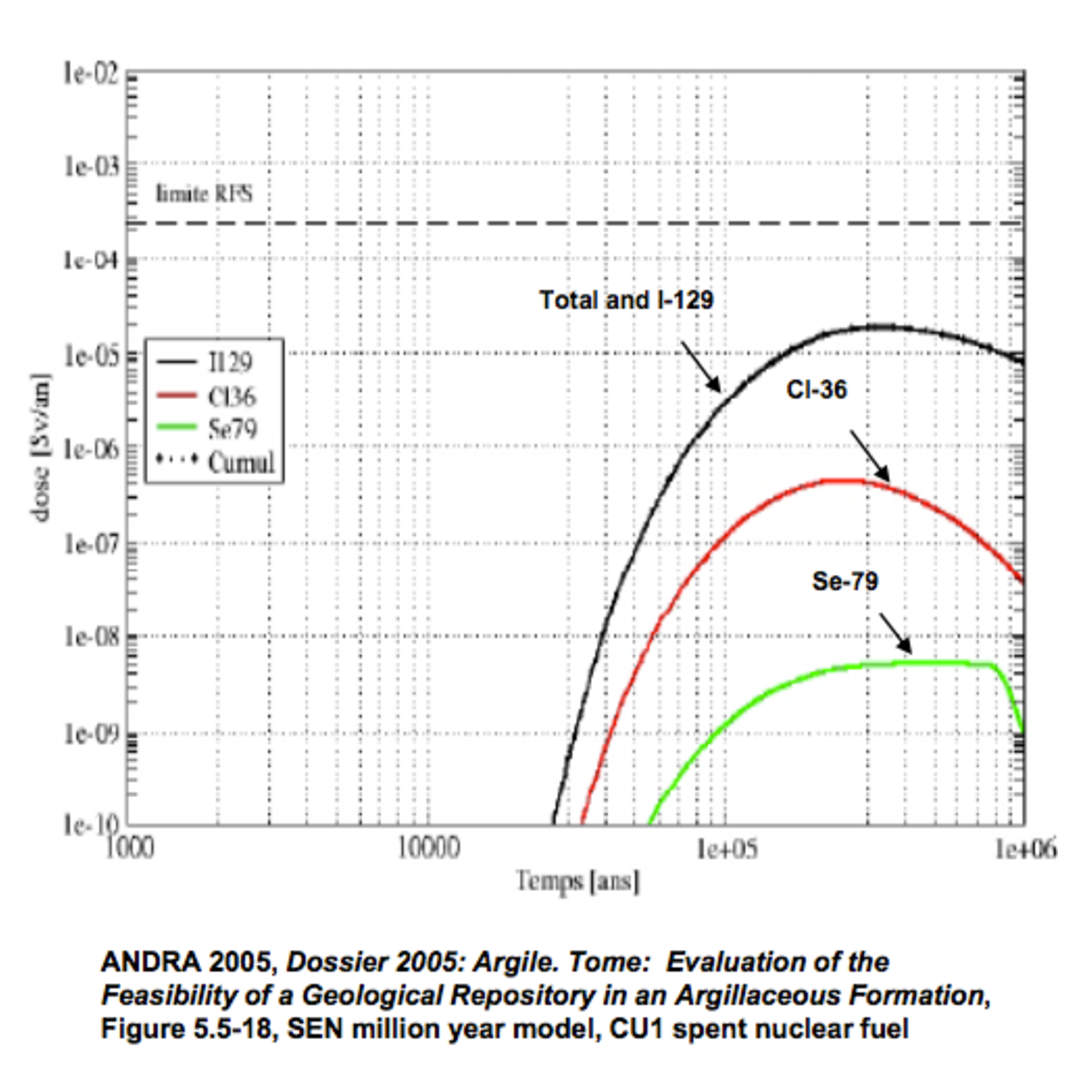
\includegraphics[width=0.7\textheight]{swift_clay_dose.eps}
  \end{center}
  \caption{Dose contributors expected in a clay repository concept 
    \cite{swift_applying_2010}.}
  \label{fig:swift_clay_dose}
\end{figure}

}
\end{frame}

%%----------------------------------------%%
\begin{frame}[ctb!]
  \frametitle{Dose Contributors, PWR SNF In Granite}
\footnotesize{
  \begin{figure}[htbp!]
  \begin{center}
    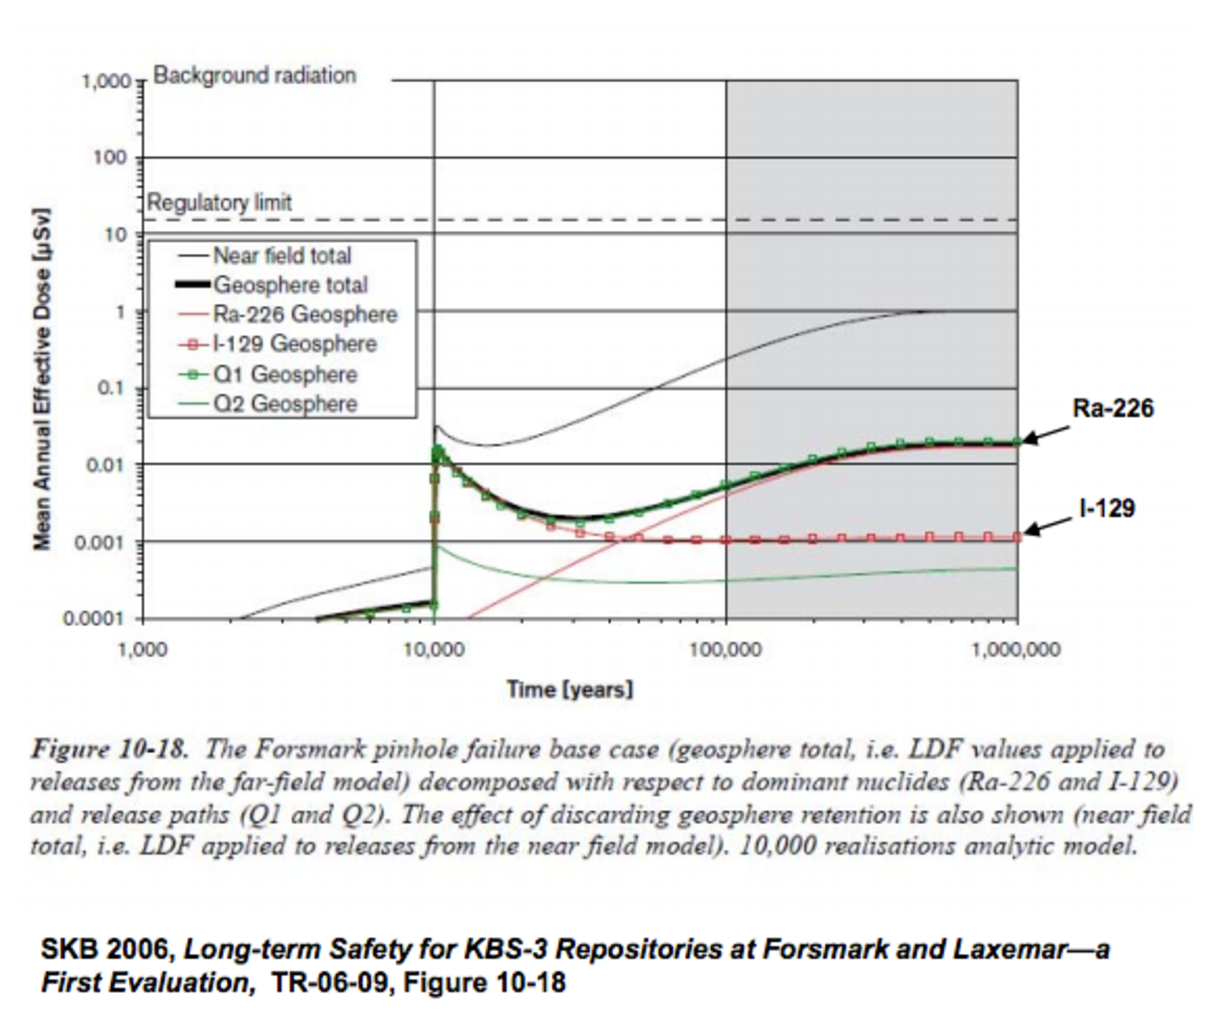
\includegraphics[width=0.7\textheight]{swift_granite_dose.eps}
  \end{center}
  \caption{Dose contributors expected in a granite repository concept 
    \cite{swift_applying_2010}.}
  \label{fig:swift_granite_dose}
\end{figure}

}
\end{frame}


\subsection{Other Factors}

%%----------------------------------------%%
\begin{frame}[ctb!]
\footnotesize{
  \frametitle{<++>}
  <++>
}
\end{frame}

%%----------------------------------------%%
\begin{frame}[ctb!]
\footnotesize{
  \frametitle{<++>}
  <++>
}
\end{frame}



%%----------------------------------------%%
\begin{frame}[ctb!]
  \frametitle{Conclusion}
  Thanks!
  
  Feel free to direct questions to huff2@wisc.edu.
\end{frame}

%%--------------------------------%%
%%--------------------------------%%
\begin{frame}[allowframebreaks]
  \frametitle{References}
  \bibliographystyle{plain}
  {\footnotesize \bibliography{ne571} }

\end{frame}

%%--------------------------------%%




\end{document}



